\documentclass[a4paper,12pt]{ctexart} %A4纸,小四号字体
\usepackage{ctex}

\usepackage{geometry} 
\geometry{left=3.17cm,right=3.17cm,top=2.54cm,bottom=2.54cm} %上下左右空白距离
\pagestyle{plain}
\usepackage{titlesec} %标题
\usepackage{setspace}
\usepackage{enumerate}
\usepackage{parskip} % Package to tweak paragraph skipping 
\usepackage{tikz} % Package for drawing 
\usepackage{amssymb}%数学字体与符号 
\usepackage{amsmath}%数学公式 
\usepackage{hyperref}%超链接与其他 PDF 专有功能(如表单制做)常用 
\usepackage{booktabs}%使用三线表booktabs 
\usepackage{threeparttable}
\usepackage{tabularx}
\usepackage{longtable}%长表格自动分页 
\usepackage{graphicx}%插入图片 
\usepackage{subfigure} %多张图片组合
\usepackage{float}%将图片插入指定位置[H] 
\usepackage{indentfirst}%首行缩进
\setlength{\parindent}{2em} %段首缩进
\setlength{\parskip}{0em} %段落间距
\usepackage{times} %使得英文默认字体都是Times New Roman
\usepackage{verbatim}
\usepackage{gensymb}
\usepackage{listings}
\usepackage{xcolor}
\linespread{1.3} %全文行间距

\newcommand{\song}{\CJKfamily{song}}
\newcommand*{\dif}{\mathop{}\!\mathrm{d}}

\titlespacing*{\section} {0pt}{3pt}{6pt} %一级标题间距
\titlespacing*{\subsection} {0pt}{0pt}{0pt} %二级标题间距
\titlespacing*{\subsubsection} {0pt}{0pt}{0pt} %三级标题间距
\titleformat{\section}[block]{\centering\large\bfseries}{\arabic{section}}{1em}{}
\titleformat{\subsection}[block]{\normalsize\bfseries}{\arabic{section}.\arabic{subsection}}{0.5em}{}
%章节序号与标题的字号及间距修改
\titleformat{\subsubsection}[block]{\normalsize\bfseries}{\arabic{section}.\arabic{subsection}.\arabic{subsubsection}}{0.5em}{}
\renewcommand{\arraystretch}{1.5} %控制行高
\definecolor{dkgreen}{rgb}{0,0.6,0}
\definecolor{gray}{rgb}{0.5,0.5,0.5}
\definecolor{mauve}{rgb}{0.58,0,0.82}
\lstset{
	frame=tb,
	aboveskip=3mm,
	belowskip=3mm,
	showstringspaces=false,
	columns=flexible,
	framerule=1pt,
	rulecolor=\color{gray!35},
	backgroundcolor=\color{gray!5},
	basicstyle={\small\ttfamily},
	numbers=none,
	numberstyle=\tiny\color{gray},
	keywordstyle=\color{blue},
	commentstyle=\color{dkgreen},
	stringstyle=\color{mauve},
	breaklines=true,
	breakatwhitespace=true,
	tabsize=3,
}
\begin{document}
	\title{炉温曲线\vspace{-3em}}
	\date{}
	\maketitle
	\section*{摘要}
	本文研究建立回焊炉炉温曲线模型,求解相关问题,从机理模型角度研究炉内温度变化规律,对于指导制定焊接工艺流程具有重要意义。\par
	问题一要求建立焊接区域温度变化模型,求解焊接区域过回焊炉炉时不同时空下的温度。设立简化坐标系,将泛炉内加热区温度与过炉速度作为参数分析。建立二维稳态传热方程,通过分析传热方式建立边界约束条件,使用集总参数分析得出目标函数$t_\tau$。结合二维传热方程、边界条件、目标函数建立温度变化模型。采用五点菱形差分法迭代求解,利用三分法遍历得到最优时间常数 $\tau_c$=47.9567,代入数据得到炉温曲线图,求解得到温区 3,6,7中点和温区 8结束点温度分别为 141.06°C,172.78°C,191.01°C和 223.22°C。\par
	问题二要求根据设定的小温区温度求解最大过炉速度。本文对温度变化斜率、温度处于150$\sim$190°C时长、超过 217°C时长和峰值温度为 240$\sim$250°C等制程界限进行离散化表达。采用定步长遍历法,求得最大过炉速度为 72.25cm/min并得到炉温曲线。\par
	问题三要求在超过 217°C到峰值温度所覆盖面积最小的情况下,求解最优炉温曲线、过炉速度及各温区设定温度。以最小化阴影面积为目标函数,使用制程界限及题干焊接区域中心温度界限为约束,建立单目标优化模型。采用遗传算法迭代,求得最优炉温曲线,对应最小阴影面积指标为461.14。温区 1$\sim$5,6,7, 8$\sim$9温度分别为 179.59°C,203.12°C,244.49°C和 265.00°C,传送带过炉速度为99.98cm/min。\par
	问题四以最小化阴影面积S 和对称度E为目标函数,确立制程界限与决策变量向量,建立多目标优化模型。采用多目标遗传算法NSGA-II,运用Matlab迭代得到Pareto前沿图,求得最优对称度指标为2.5,最小化面积指标为469.24,对应温区1$\sim$5,6,7,8$\sim$9温度分别为167.72°C,191.99°C,228.72°C和265.00°C,传送带速度为88.16cm/min。\par
	\noindent\textbf{关键词}:\textbf{集总参数分析}\quad  \textbf{五点菱形差分}\quad   \textbf{三分法}\quad \textbf{多目标遗传算法NSGA-II}\quad
	\newpage
	\section{问题背景及重述}
	\subsection{问题背景及相关信息}
	回焊炉是一种主要用于生产集成电路板等电子产品的设备,它可以通过加热将电子元件自动焊接到电路板上。回焊炉内部设有不同小温区,在功能上分类可将其分成预热区,恒温区,回流区与冷却区4个大温区。工作时通过把电路板两侧搭上传送带进炉加热焊接。\par
	当不同温区与传送带的温度设置完毕,可使用温度传感器测量某些位置上焊接区域中心的温度并形成炉温曲线(焊接区域中心温度曲线)。在电路板的焊接生产中,炉温曲线应该满足一定的制程界限。\par
	在上述实验设定温度的基础上,各小温区设定温度可以进行$\pm$10°C范围内的调整。调整时要求小温区1$\sim$5中的温度保持一致,小温区8$\sim$9中的温度保持一致,小温区10$\sim$11中的温度保持25°C。传送带的过炉速度调节范围为65$\sim$100 cm/min。\par
	\subsection{问题重述}
	1.给定传送带过炉速度为78cm/min,各温区温度的设定值分别为173°C(小温区1$\sim$5)、198°C(小温区6)、230°C(小温区7)和257°C(小温区8$\sim$9)。根据以上数据建立有关焊接区域温度变化规律的数学模型,同时给出区域中心的温度变化情况,列出小温区3、6、7中点及小温区8结束处焊接区域中心的温度,画出相应的炉温曲线,并将每隔0.5s焊接区域中心的温度存放在提供的result.csv中。\par
	2.设定各温区温度分别为182°C(小温区1$\sim$5)、203°C(小温区6)、237°C(小温区7)、254°C(小温区8$\sim$9),就这些数据得出允许的最大传送带过炉速度。\par
	3.已知在焊接过程中,焊接区域中心的温度高于217°C的时间不宜过长,峰值温度也不宜过高。在炉温曲线上表现为超过217°C到峰值温度所覆盖的面积最小。需要确定在该要求下的最优炉温曲线,各温区的设定温度和传送带的过炉速度,并给出相应的覆盖面积。\par
	4.为了使焊接完成的产品质量保持较高水准,除了考虑要求的制程界限,还应使峰值温度为中心线的两侧超过217°C的炉温曲线尽量对称。结合问题3,进一步给出最优炉温曲线,各温区设定的温度及传送带过炉速度,并给出相应的指标值。\par
	\section{问题假设}
	\begin{itemize}
		\item 假设回焊炉内部没有自发热源存在
		\item 假设上下区各对应加热温区参数均相同
		\item 假设各温区工作时不会发生自发热量传递
		\item 假设炉内原件不会因为持续工作发生损耗进而性能下降。
		\item 假设电路板材料不会因为经过不同温度区域而发生性质上的改变。
	\end{itemize}
	\section{符号说明}
	\renewcommand{\arraystretch}{1.5} %控制行高
	\begin{table}[h]
	\centering
	\newcolumntype{C}[1]{>{\centering\arraybackslash}p{#1}}
		\begin{tabular}{C{3cm}C{7cm}C{3cm}}
			\toprule
			符号 & 说明 & 量纲\\ \midrule
			$\tau$  & 时间& s\\
			$\tau_c$  & 时间常数 & °C\\
			$\boldsymbol{x}$&决策变量&/ \\
			$t_{I}$ ,$t_{II}$,$t_{III}$,$t_{IV}$  & 温区温度& °C \\ 
			$v$  & 传送带运行速度 & cm/min \\
			$x_i,y_j$  & 节点横纵坐标数值& 1\\
			$u$ & 泛炉内加热区温度& °C\\
			$L,H$ & 泛炉内加热区长与宽& cm\\
			$t_0,t_f$  & 初始温度,环境温度& °C\\
			$t$  & 区域中心随传送带在不同位置温度 & °C\\
			\bottomrule 
		\end{tabular}
	\end{table}\par
	\section{问题分析}
	\subsection{问题一的分析}
	本题要求建立焊接区域温度变化的模型,在给定过炉速度和设定各温区温度条件下,求解焊接区过炉时不同时空下的温度。首先界定泛炉内加热区范围(包含炉前区和炉内加热区),基于热力学原理,对不同区域传热规律进行探究。其二,在此基础上建立二维传热方程、边界条件,采用集总参数法建立目标函数,建立炉温数学模型,求解炉温曲线及相应温度。\par
	\subsection{问题二的分析}
	本题要求根据设定的小温区温度求解最大传送带过炉速度,其本质是一道优化问题。首先由于问题一求解为离散型解,延续前题对制程界限进行离散化表达;然后,基于题干所求为最大值,使用定步长遍历法算法,求解最大过炉速度。 \par
	\subsection{问题三的分析}
	本题要求在超过217°C到峰值温度所覆盖面积最小的情况下求解最优炉温曲线、过炉速度及各温区设定温度。与问题二类似,本题亦是一道单目标优化问题。首先以制程界限及焊接区域中心温度界限为约束,建立以最小化阴影面积为目标的单目标优化模型;其次由于变量多、函数复杂等因素,迭代得到最优炉温曲线等目标。\par
	\subsection{问题四的分析}
	本题要求在峰值中心线的两侧超过217C的炉温曲线尽量对称的情况,求解最优炉温曲线等问题,其本质是多目标优化问题。首先以最小化阴影面积S 和对称度H为目建立多目标优化模型。然后迭代求得最小化阴影面积、最优对称度,相应求得各小温区设定温度等目标。\par
	
	\section{模型的建立与求解}
	
	\subsection{问题一模型建立与求解}
	已知在实际生产中回焊炉为一个三维物体\cite{ref1},为了简化理解,本文首先做出截面示意图,并以炉前区域左端到传送带上投影点为原点,以传送带为x轴,以炉前左端纵向方向为y轴向建立直角坐标系如图1:\par
		\begin{figure}[H]
		\centering
		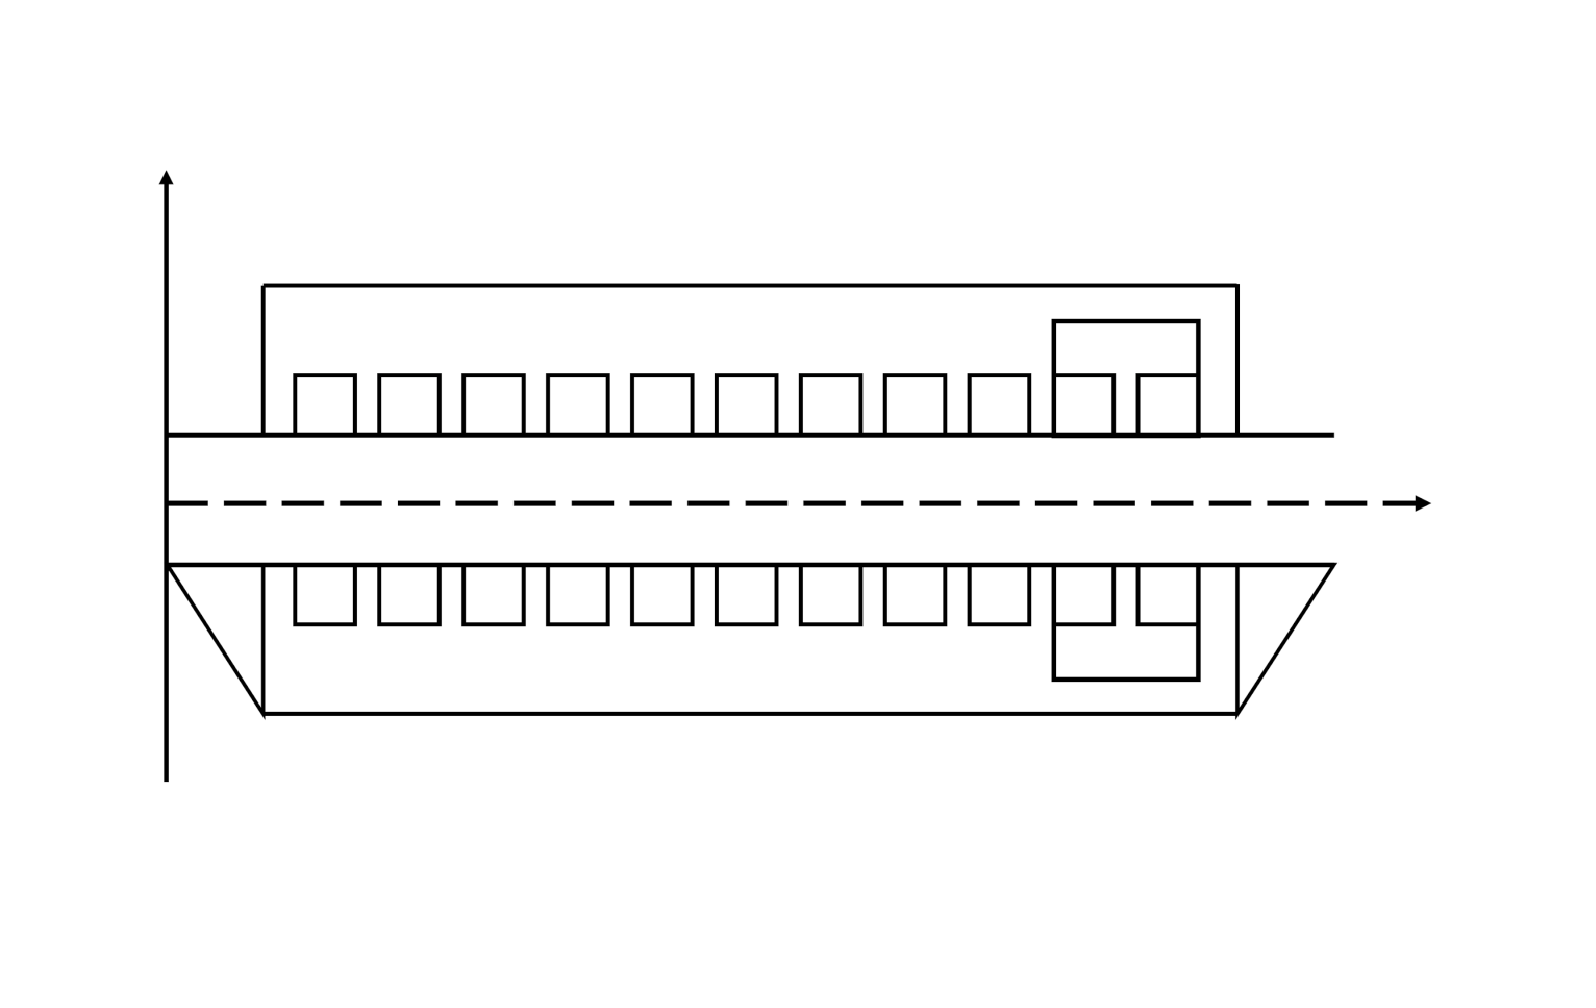
\includegraphics[scale=0.3]{Q1-1}
		\caption{回焊炉截面示意图}
	\end{figure}\par
	针对问题一,需要建立模型求解电路板焊接中心的温度变化,直观反映即为炉温曲线。本文确定泛炉内加热区域环境温度和传送带运行速度为炉温曲线的主要影响因素,对此分别进行分析。\par
	\subsubsection{泛炉内加热区分析}
	上下两排小温区中间的区域即为泛炉内加热区,该区域包括炉前区和炉内加热区,其形状为矩形,四边界定义如下:上、下两长边(设定为$L_u,L_d$),分别以上、下两排小温区朝向炉膛内的边界为长边;左宽边(设定为$H_l$)为炉前区左边与上下两长边的截断,右宽边(设定为$H_r$)为小温区9、10间隙中间的上下连线,具体位置如下图2蓝线所界定的区域:
		\begin{figure}[H]
		\centering
		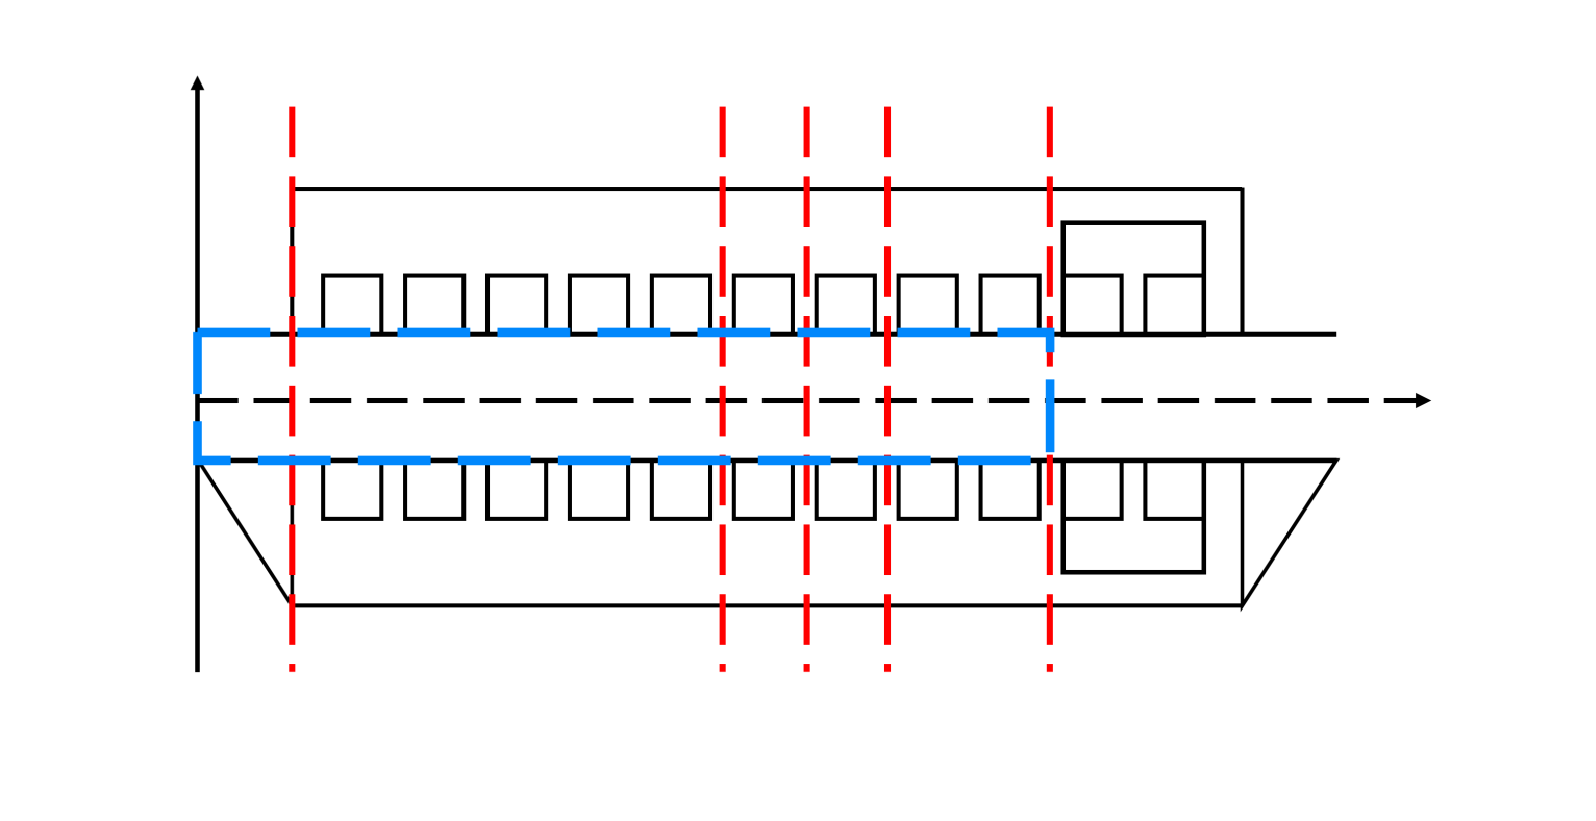
\includegraphics[scale=0.3]{Q1-2}
		\caption{中间区域示意图}
	\end{figure}\par
	对于该区域,由于回焊炉开始工作时其内部空气温度保持一个稳定值,区域内无自发热源且区域,可以将该区域视为稳态区域。而所在平面用二维方式表示,即可根据直角坐标系建立二维稳态传热方程如下\cite{ref2}:
	\begin{equation}\label{e1}
	\dfrac{\partial u}{\partial\tau}=\alpha\left(\dfrac{\partial^2 u}{\partial x^2}+\dfrac{\partial^2 u}{\partial y^2}\right)
	\end{equation}\par
	区域为稳态,即$\dfrac{\partial u}{\partial\tau}=0$,因此有:
	\begin{equation}
	\dfrac{\partial^2 u}{\partial x^2}+\dfrac{\partial^2 u}{\partial y^2}=0
	\end{equation}\par
	\subsubsection{炉内加热区边界条件建立}
	除传热微分方程外,泛炉膛加热区与周边环境之间存在热量传导,这会影响区域温度分布状态,须针对此情况进行分析。\par
	区域边界包含两条宽边$H_l,H_r$与两条长边$L_u,L_d$,现在分别进行解释。其中$H_l$与坐标系y轴重合,原因在于炉前区域温度受到临近的小温区一影响无法到达相对稳态。其外部接触25°的室内环境,内部接触炉前区域。对于$H_r$由于冷却区(即小温区10,11)温度固定在25°与室温相同,选择小温区9与小温区10的边界作为该宽边。其外部接触25°冷却区环境,内部接触257°小温区9。\par
	对上下两长边$L_u,L_d$,其由不同类型边界组成,包括炉前区域边、1$\sim$9小温区边以及小温区间隙边。这些边对应温度变化也不尽相同:1$\sim$9小温区边,其温度与对应小温区相同;1$\sim$5小温区间隙温度恒定,8$\sim$9小温区间隙温度恒定;炉前区域,5,6小温区间隙, 6,7小温区间隙和 7,8小温区间隙,其共同特征为两端温度不等,需要通过二维稳态传热方程求解。由这些间隙边水平可知$\frac{\partial^2 u}{\partial y^2}=0$,所以$u$是一个关于横坐标$x$的线性函数。具体长边温度随位置横坐标变化与中心线对比图如图3:
	\begin{figure}[H]
		\centering
		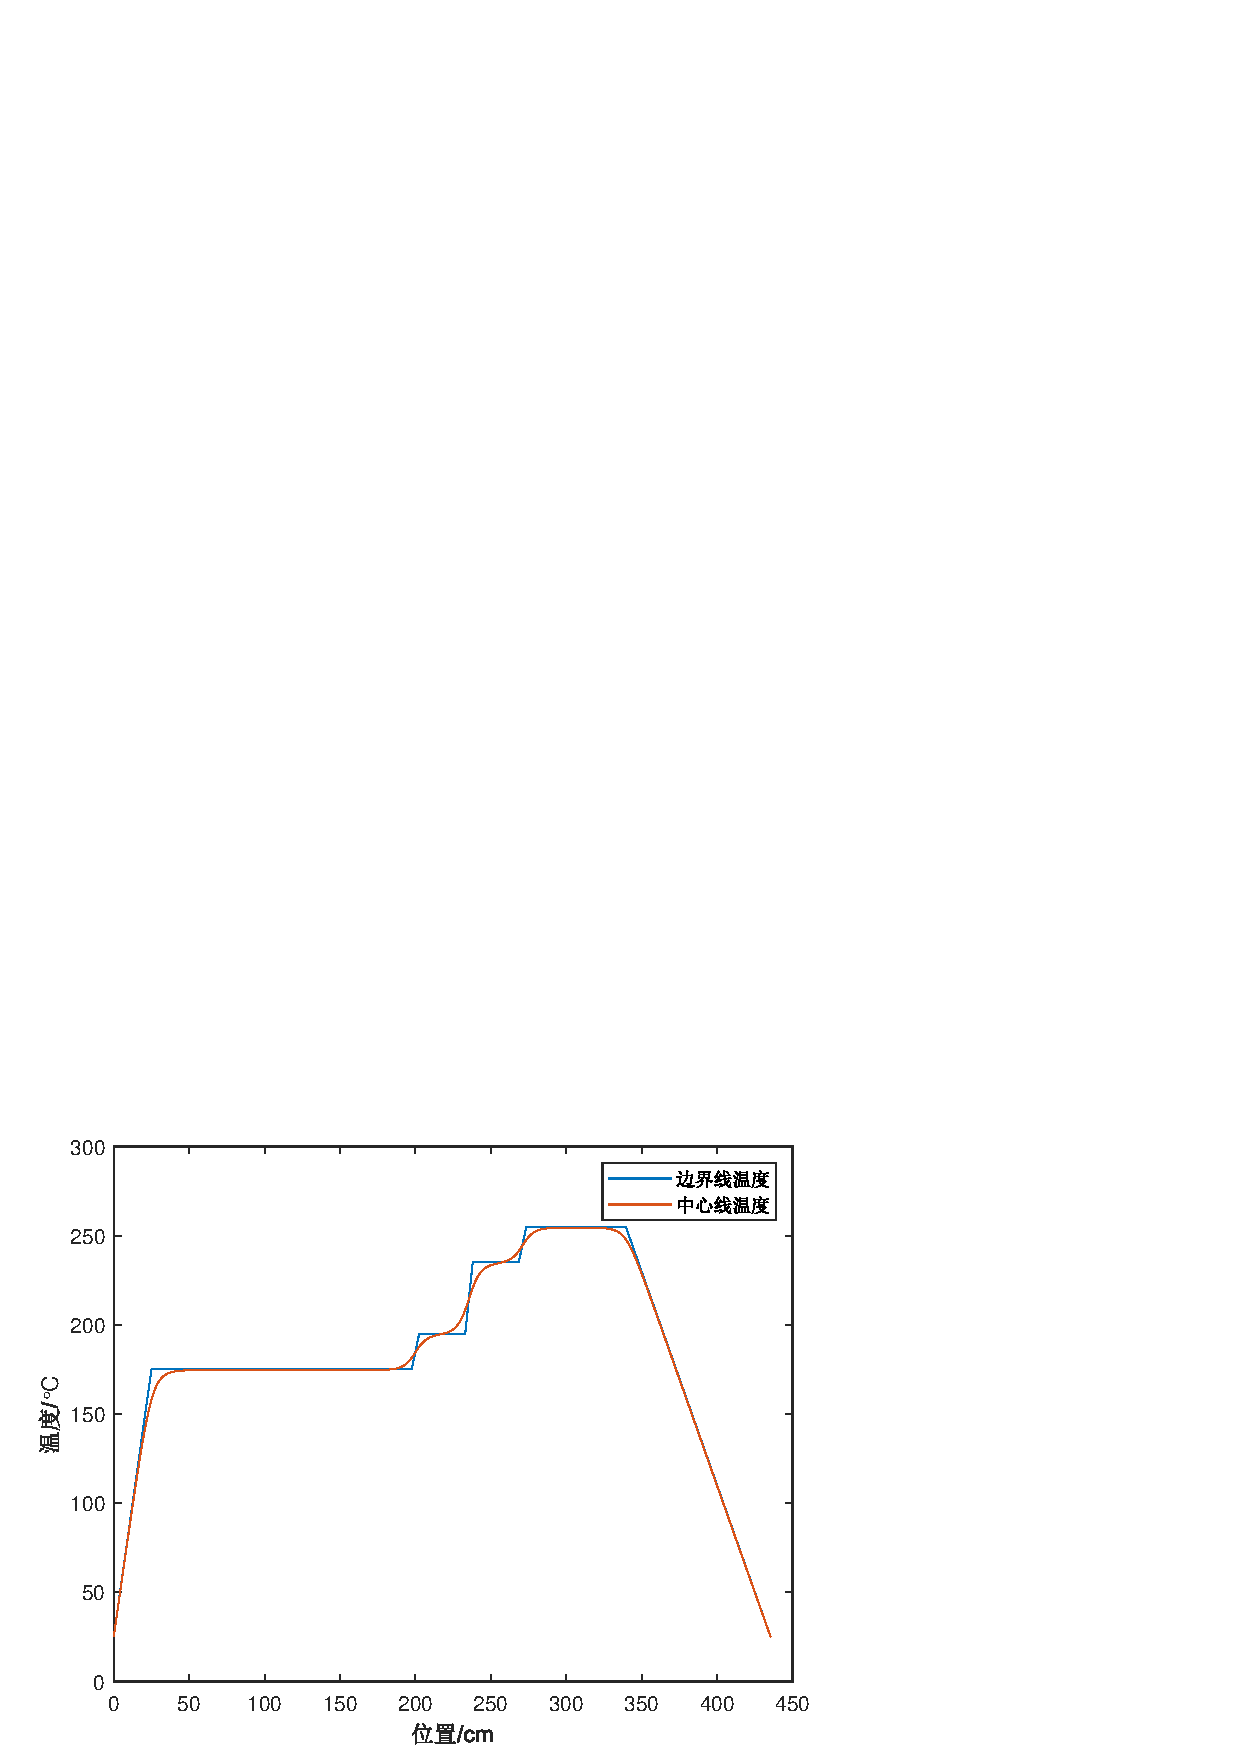
\includegraphics[scale=0.6]{Q1-edge}
		\caption{边界条件与中心线温度对比图}
	\end{figure}\par
	现对边界条件进行具体的数学表述,记温度表达式为$u\left(x,y\right)$,其中$x,y$分别代表位置横纵坐标。由上文所述$H,L$条件有:
	\begin{equation}
	\begin{cases}
	u\left(x,-\dfrac{d}{2}\right)=u\left(x,\dfrac{d}{2}\right)=u_b\left(x\right)\\
	u\left(0,y\right)=u\left(l,y\right)=25\degree\mathrm C\\
	\end{cases}
	\end{equation}
	\subsubsection{ 传送带速度分析}
	前两节分析了泛炉内加热区环境温度,现在分析传送带速度对于炉温曲线的影响。\par
	已知传送带过炉速度恒定,它带动挂在上面需要焊接的电路板匀速运动,即焊接中心沿传送带依次经过不同温度区域,所以可视其为非稳态过程。对此使用集总参数方法\cite{ref2},其本质在于将物体近似处理成为一个质点,忽略其实际体积,质量,且在同一时刻只有一个温度值。对应其解的形式为:
	\begin{equation}
	t=f\left(\tau\right)
	\end{equation}\par
	本文以能量平衡作为着手点,将能量平衡运用到物体冷却过程中:
	\begin{equation}
	-\rho cV\dfrac{\mathrm{d}t}{\mathrm{d}\tau}=hA\left(t-t_f\right)
	\end{equation}\par
	其中$\rho$代表物体密度,$c$代表比热容,$V,A$分别代表表面积和体积,$t_f$为环境温度,$h$为对流换热系数。本式说明空气吸收热流量等于物体降温释放的热流量。令过余温度$\theta=t-t_f$,上式变为:
	\begin{equation}\label{e2}
	-\rho cV\dfrac{\mathrm{d}t}{\mathrm{d}\tau}=hA\theta
	\end{equation}\par
	对应的初始条件可以表达成:
	\begin{equation}\label{e3}
	\theta\left(0\right)=t_0-t_f=\theta_0
	\end{equation}\par
	使用分离变量法,对式\ref{e2}与式\ref{e3}求其定解:
	\begin{equation}
	\int_{\theta_0}^{\theta}\dfrac{\mathrm{d}\theta}{\theta}=-\int_{0}^{\tau}\dfrac{hA}{\rho cV}\mathrm{d}\tau
	\end{equation}\par
	对以上微分式积分并且表达为指数函数:
	\begin{equation}
	\frac{\theta}{\theta_0}=\frac{t-t_f}{t_0-t_f}=e^{-\frac{hA}{\rho cV}\tau}
	\end{equation}\par
	最后得出$t$的表达式为:
	\begin{equation}
	t=\left(t_0-t_f\right)e^{-\frac{hA}{\rho cV}\tau}+t_f
	\end{equation}\par
	现将$\frac{\rho cV}{hA}$记为时间常数$\tau_c$,$t$的表达式变为:
	\begin{equation}\label{e4}
	t=\left(t_0-t_f\right)e^{-\frac{\tau}{\tau_c}}+t_f
	\end{equation}\par
	由于本题所求为数值解,在此给出一种温度变化函数$t_{\tau}$的数值解微分求法。\par 取$\tau=0$附近微小变量$\varDelta t$,可得:
	\begin{equation}
	\varDelta t=t'_{\tau}\bigg|_{\tau=0}
	\end{equation}\par
	由于$\varDelta t$微小,可近似边界温度$t_f$在保持不变。代入t表达式\ref{e4},得到下式:
	\begin{equation}
	\varDelta t=\left(t-t_f\left(v\tau\right)\right)\left(-\frac{1}{\tau_c}\right)\varDelta\tau
	\end{equation}\par
	化为微分式为:
	\begin{equation}
	\mathrm{d} t=\left(t-t_f\left(v\tau\right)\right)\left(-\frac{1}{\tau_c}\right)\mathrm{d}\tau
	\end{equation}\par
	代具体点入该式积分即可得到对应$t_{\tau}$。
	\subsubsection{问题一模型建立}
	所需目标函数即焊接区域中心温度变化函数$t\left(\tau\right)$。约束条件即二维传热稳态方程和边界条件。有:
	\begin{equation}
	s.t.\begin{cases}
	\dfrac{\partial^2 u}{\partial x^2}+\dfrac{\partial^2 u}{\partial y^2}=0\\[1em]
	u\left(x,-\dfrac{d}{2}\right)=u\left(x,\dfrac{d}{2}\right)=u_b\left(x\right)\\[1em]
	u\left(0,y\right)=u\left(l,y\right)=25\degree\mathrm C\\[1em]
	t=\left(t-t_f\left(v\tau\right)\right)\left(-\frac{1}{\tau_c}\right)\mathrm{d}\tau\\
	\end{cases}
	\end{equation}
	由以上条件可求出区域中心温度变化。\par
	
	\subsubsection{问题一模型求解}
	二维稳态导热式\ref{e1}为二维椭圆形方程中的拉普拉斯方程,由于约束条件方程较为复杂,因此不解析求方程精确解,而是求数值解\cite{ref3}。求解时的方法包括五点菱形差分,九点紧差分等。\par
	本问题采用五点菱形差分的方法处理,思路在于结合二维稳态导热方程与边界条件,将原来连续区域刨分成为离散性区域,使方程仅在离散点成立,同时将方程中微商用差商代替得到数值解,具有高效性精确性等优点,具体步骤如下:\par
	1.分割矩形区域,在x方向进行步长为$\varDelta x$等距剖分,分为m份。即$\varDelta x=l/m$,$l$为长度$L$具体值,同时在y方向进行步长为$\varDelta y $等距剖分,分为n份。即$\varDelta y=d/n$,$d$为中间区域宽度$H$具体值。\par
	可知对应节点横坐标纵坐标分别为:
	\begin{equation}
	\begin{cases}
	x_i=i\cdot \varDelta x\quad\quad i=0,1,2\dots m\\
	y_j=-\frac{d}{2}+j\cdot \varDelta y\quad\quad j=0,1,2\dots n \\
	\end{cases}
	\end{equation}\par
	在此基础上可以把该中间区域分为$mn$个小矩形,并得到节点$\left(x_i,y_j\right)$。\par
	2.将二位稳态导热方程弱化,使之只在离散的节点成立,对应下式:
	\begin{equation}
	\begin{cases}
	\left(\dfrac{\partial^2 u}{\partial x^2}+\dfrac{\partial^2 u}{\partial y^2}\right)\bigg|_{\left(x_i,y_j\right)}=0\quad\quad \left(x_i,y_j\right)\in\varOmega^o\\[1em]
	u\left(x,-\frac{d}{2}\right)=u\left(x,\frac{d}{2}\right)=u_b\left(x\right)\\
	u\left(0,y\right)=u\left(l,y\right)=25\degree\mathrm C\\
	\end{cases}
	\end{equation}\par
	3.再用差商近似取代微商,创建数值格式的方程如下,这里将$\varDelta x^2,\varDelta y^2$分别记为$h^2,k^2$:
	\begin{equation}
	\begin{cases}
	\dfrac{\partial^2 u}{\partial x^2}\bigg|_{\left(x_i,y_j\right)}=\dfrac{u\left(x_{i-1},y_j\right)-2u\left(x_i,y_j\right)+u\left(x_{i+1},y_j\right)}{h^2}+O\left(h^2\right)\\[1em]
	\dfrac{\partial^2 u}{\partial y^2}\bigg|_{\left(x_i,y_j\right)}=\dfrac{u\left(x_i,y_{j-1}\right)-2u\left(x_i,y_j\right)+u\left(x_i,y_{j+1}\right)}{k^2}+O\left(k^2\right)\\
	\end{cases}
	\end{equation}\par
	代入离散节点处方程,用数值解$u_{i,j}$代替精确解$u\left(x_i,y_j\right)$,取四个边中点计算,忽略高阶小项可得到数值格式:
	\begin{equation}
	\begin{cases}
	\dfrac{u_{i-1,j}-2u_{i,j}+u_{i+1,j}}{h^2}+\dfrac{u_{i,j-1}-2u_{i,j}+u_{i,j+1}}{k^2}=0\\[1em]
	\quad\quad 1\leqslant i\leqslant m-1,1\leqslant j\leqslant n-1\\
	u_{i,j}=t\left(x_a,y_b\right)\quad a=0,m\quad b=\pm \frac{d}{2}
	\end{cases}
	\end{equation}\par
	该式的局部截断误差为$O\left(h^2+k^2\right)$。上式整理得:
	\begin{equation}
	\begin{cases}
	 h^2\left(u_{i-1,j}+u_{i+1,j}\right) + k^2\left(u_{i,j-1}+u_{i,j+1}\right) -2\left(h^2+k^2\right)u_{i,j} = 0\\
	\quad\quad 1\leqslant i\leqslant m-1,1\leqslant j\leqslant n-1\\
	u_{i,j}=u\left(x_a,y_b\right)\quad a=0,m\quad b=\pm \frac{d}{2}
	\end{cases}
	\end{equation}\par
	4.这是一个高阶稀疏矩阵方程。理论上可以直接解该方程得到仿真结果,由于阶数过高本方程选用迭代方法求解。在此使用收敛速度较快的SOR迭代:
	\begin{equation}
	u_{i,j}^{(k+1)} = (1-\omega)u_{i,j}^{(k)} + \omega \frac{h^2(u_{i-1,j}^{(k+1)}+u_{i+1,j}^{(k)}) + k^2(u_{i,j-1}^{(k+1)}+u_{i,j+1}^{(k)})}{2(h^2+k^2)}
	\end{equation}\par
	其中加括号的上标$k$代表迭代次数,$0<\omega<2$。\par
	5.在迭代一定次数或误差小于一定阈值时,迭代终止,将最终得到的$u^{k+1}$作为求解的$t$的结果。\par
	取$t_f(x) = u(x,0) = u_{i,\lceil n/2 \rceil}$,将$y=0$的线上作为焊接材料在回焊炉中移动时的环境。这样取到的$t_f(x)$也是离散的点,将其记为$(t_f)_i = t_f(x_i)$。\par
	同样,对焊接原件进入回焊炉这一过程也进行离散。在时刻$\tau$取短时间段$\varDelta \tau$,由式\ref{e5},其对应一个$\varDelta t = t_i - t_{i-1}$,其中$t_i$为炉温曲线$t(\tau)$的离散形式,可以得到如下的$t_i$的计算式:
	\begin{equation}
	t_i = t_{i-1} + (t_{i-1} - (t_f)_j)(-\frac{1}{\tau_c}) \varDelta \tau
	\end{equation}\par
	其中$j$满足$x_{j-1} <v\tau \leqslant x_{j}$,且$t_0=t(0)=25$。可得炉温曲线的离散形式。\par
	在其他因素已知情况下,需要$\tau_c$的值来确定炉温曲线。由式\ref{e4},可知$\tau_c$是反映焊点温度对环境温度响应速度的物理量。由附件数据拟合得到最优$\tau_c$。\par
	首先在大范围内进行遍历,观察$\tau_c$对拟合误差的影响。其中拟合误差使用方均根误差进行计算。得到下面的误差与$\tau_c$取值的关系图如图4。\par
	\begin{figure}[H]
		\centering
		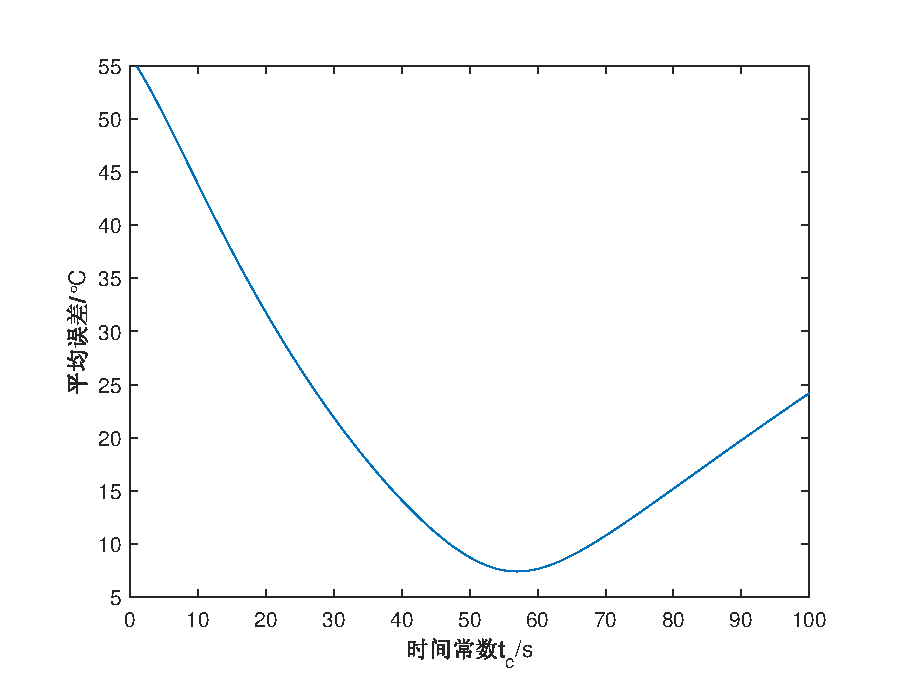
\includegraphics[scale=0.6]{Q1-3}
		\caption{时间常数$\tau_c$与误差关系图}
	\end{figure}\par
	由图可见,随着$\tau_c$的增大误差先升后降,且存在一个满足制程条件最小值位于45-65s之间。对于这种存在唯一最值的函数求最值的问题,使用三分法进行求解。其示意图如下图5,其中$err(\tau_0)$代表在$\tau_c = \tau_0$时的方均根误差:
	\begin{figure}[H]
		\centering
		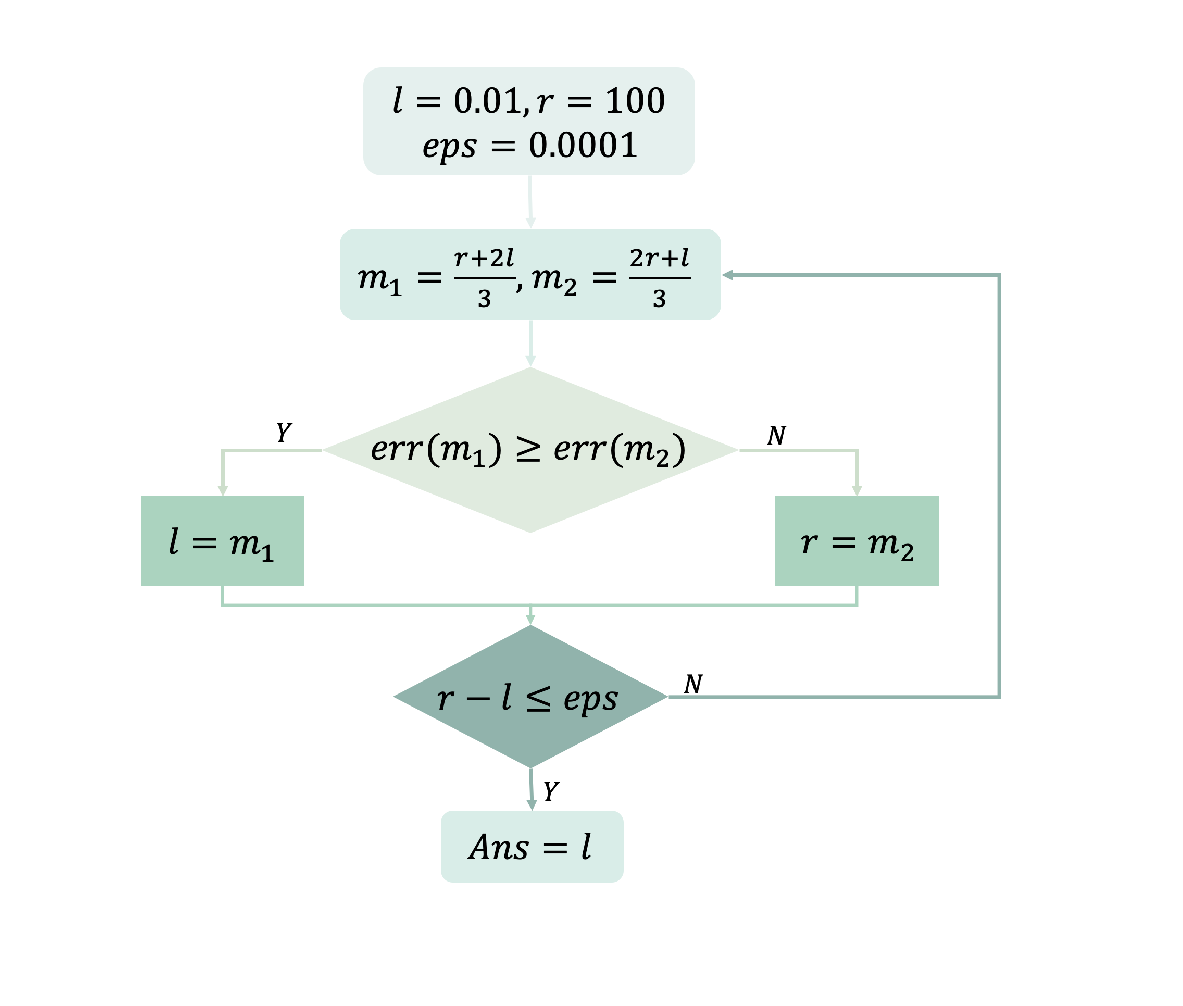
\includegraphics[scale=0.45]{Q1-4}
		\caption{三分法示意图}
	\end{figure}\par
	1.确定搜索区间左右边界$l=0.01,r=100$,确定终止阈值$eps=0.0001$;\par
	2.取区间的两个三等分点为$m_1,m_2$,其中$m_1$在$m_2$的左边。\par
	3.$err(m_1)$与$err(m_2)$比大小。若$err(m_1)\geqslant err(m_2)$,则取左边界$l=m_1$;若$err(m_1)<err(m_2)$,则取右边界$r=m_2$。\par
	4.判断$r-l$是否小于或等于$eps$值,若是,取$l$值为解,结束算法。若为否,则返回第二步。\par
	通过该方法算出最优时间常数$\tau_c=47.9567s$, 该常数值下炉温曲线与附件对比如图6:
	\begin{figure}[H]
		\centering
		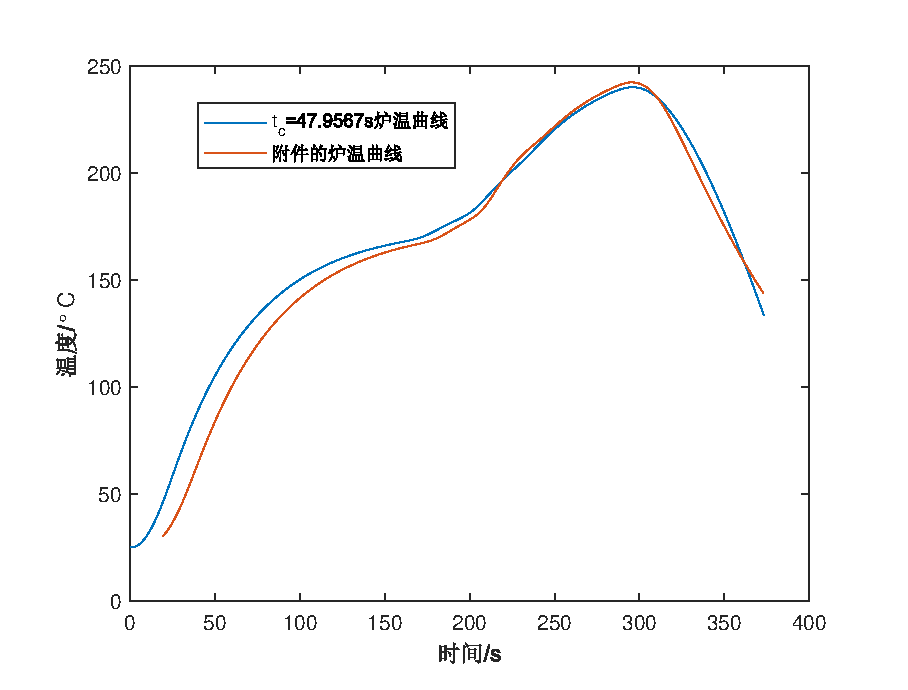
\includegraphics[scale=0.65]{Q1-5}
		\caption{炉温曲线与附件对比图}
	\end{figure}\par
	可见本文所得时间常数对应炉温曲线与附件数据误差较小。\par
	下面代入本问题所给过炉速度与温区温度等数据,得到焊接区域中心温度变化如图7:
	\begin{figure}[H]
	\centering
	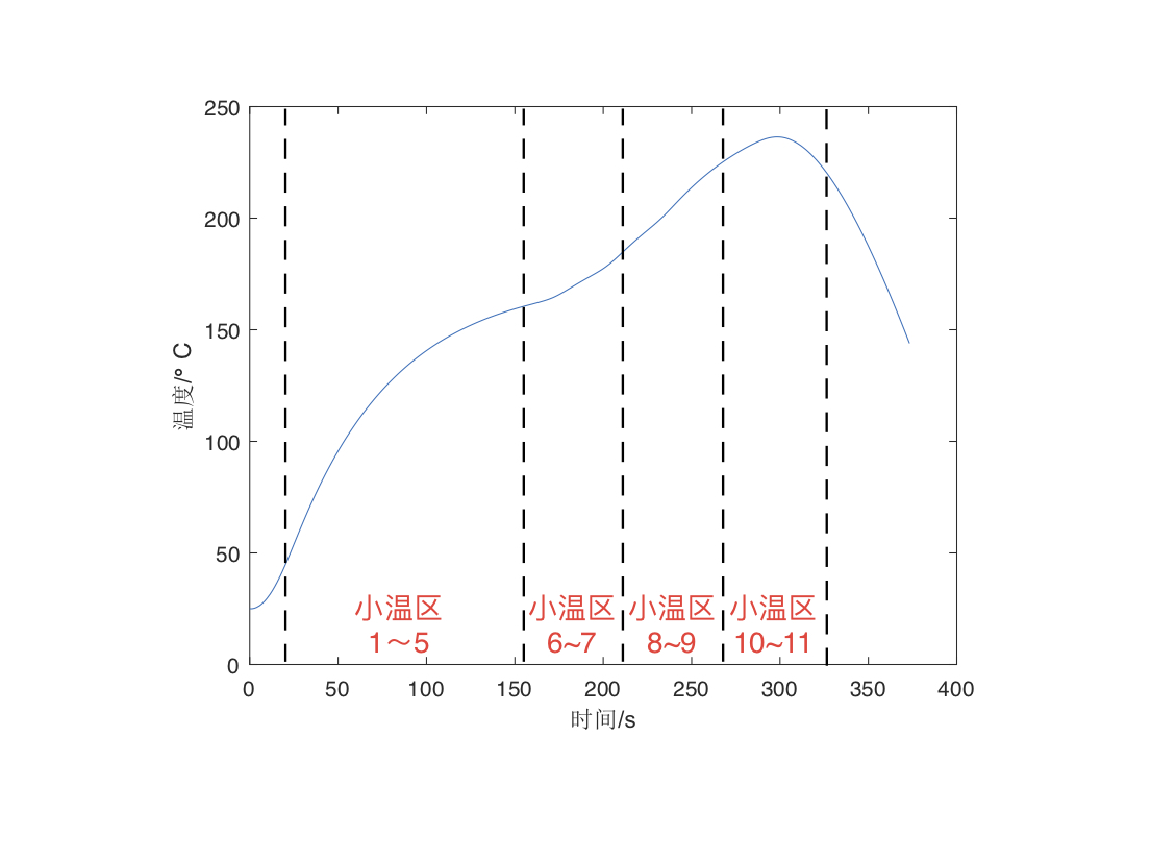
\includegraphics[scale=0.6]{Q1-6}
	\caption{焊接区域中心温度分布图}
	\end{figure}\par
	
	并给出焊接区域中心在传送带上处于与小温区3、6、7中点及小温区8结束点时的温度,对应表1:
	\begin{table}[h]
	\centering
	\caption{小温区中点温度表}
	\begin{tabular}{cc}
		\toprule
		位置& 温度(°C)\\ \midrule
		小温区3中点&141.06\\
		小温区6中点&172.78\\
		小温区7中点&191.01\\
		小温区8结束处&223.22\\
		\bottomrule 
	\end{tabular}
	\end{table}\par
	可见焊接区域中心在经过不同小温区时温度变化的趋势。根据制程界限约束条件分析,温度从1至10温区以不同的趋势上升,最大斜率为2.29,符合上升斜率在0$\sim$3的范围,温度在温区10与11交界处开始下降,其下降斜率最低值-2.38,符合下降斜率在-3$\sim$0的范围。\par
	温度上升时从温区4,5附近至温区7中点温度在150$\sim$190°C,下降时温度在150$\sim$190°C的时段位于炉后区域内,其总和经过计算为92.03s。温度处于217°C以上时的区域对应小温区9$\sim$11左右,其时长为69.90秒,两时间长度均在制程条件约束范围内。同时该温度极大值为240.17°C,符合制程界限内。\par
	
	\subsection{问题二的求解}
	问题二要求根据一组数据,在制程界限的约束下,求解传送带允许的最大过炉速度。\par
	\subsubsection{约束条件的确定}
	本题约束条件即为制程界限,由于之前所求解为离散型解,约束条件亦亦进行离散化表示。\par
	取一段关于时间的微元$\varDelta\tau$,每个微元对应一个离散型分布时间节点,现对制程界限进行解释。\par
	首先关注温度变化的斜率,制程界限要求温度变化的斜率在$[-3,3]$范围内,对应斜率表达如下:
	\begin{equation}
	-3\leqslant\frac{t_{i+1}-t_i}{\varDelta\tau}\leqslant 3
	\end{equation}\par
	其中i作为下标对应取值范围为$0\leqslant i\leqslant [\frac{L}{v\varDelta\tau}]$。(后面式中i的取值范围保持恒定)。\par
	对于温度上升过程中,温度处于150$\sim$190°C的时长,有要求在60$\sim$120s范围,表达式如下:
	\begin{equation}
	60\leqslant\sum_{t_i\in[150,190],t_{i+1}\geqslant t_i} \varDelta\tau\leqslant 120
	\end{equation}\par
	对于温度超过217°C时间规定在40$\sim$90s范围的条件,表达式如下:
	\begin{equation}
	40\leqslant\sum_{t_i>217}\varDelta\tau\leqslant 90
	\end{equation}\par
	对于峰值温度要求在240$\sim$250°C的条件,表达式如下:
	\begin{equation}
	240\leqslant\max_{i=1}^{n}\left\{t_i\right\}\leqslant 250
	\end{equation}\par
	将以上条件汇总,有:
	\begin{equation}
	s.t.\begin{cases}
	-3\leqslant\dfrac{t_{i+1}-t_i}{\varDelta\tau}\leqslant 3\\[1em]
	60\leqslant\sum\limits_{\begin{smallmatrix}
		t_i\in[150,190],\\
		t_{i+1}\geqslant t_i
		\end{smallmatrix}} \varDelta\tau\leqslant 120\\[1em]
	40\leqslant\sum\limits_{t_i>217}\varDelta\tau\leqslant 90\\[1em]
	240\leqslant\max\limits_{i=1}^{n}\left\{t_i\right\}\leqslant 250\\[1em]
	\end{cases}
	\end{equation}\par
	\subsubsection{最大过炉速度求解}
	本问使用定步长遍历进行求解。遍历之前先做出对于各约束条件在速度为65$\sim$100时取值直线,如图8:
	\begin{figure}[H]
		\centering
		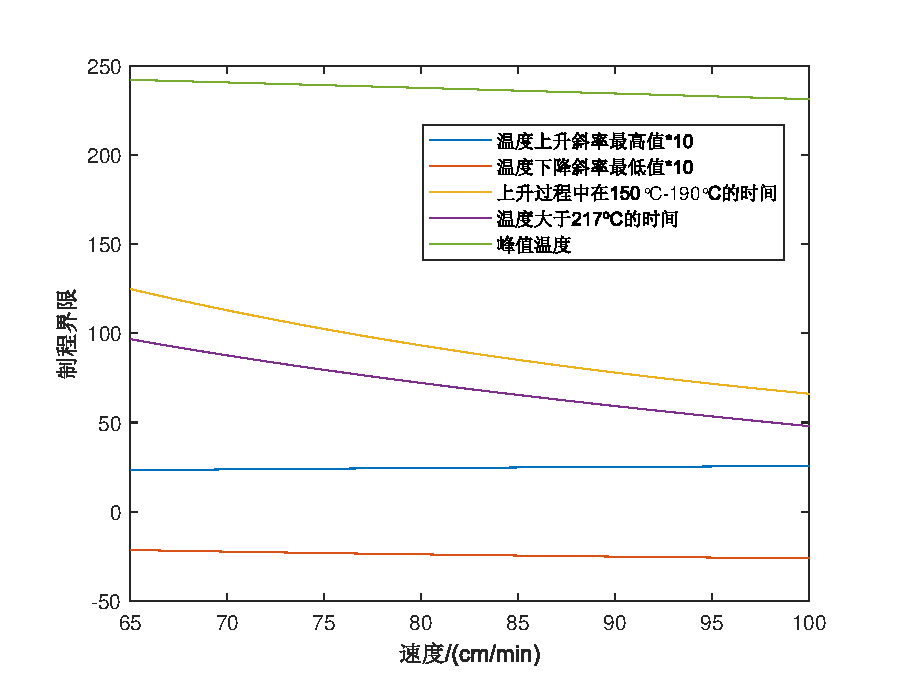
\includegraphics[scale=0.65]{Q2-1}
		\caption{不同下各约束条件制程界限图}
	\end{figure}\par
	进行遍历,由于所求为最大传送带过炉速度,先从100往65以定步长为1进行遍历,发现在70附近出现第一个符合条件值,即最大速度。\par
	再进行步长为0.01的遍历,将取值范围精确在72$\sim$73内,最终确定72.25是符合条件最大速度,其对应炉温曲线如图9:\par
	\begin{figure}[H]
		\centering
		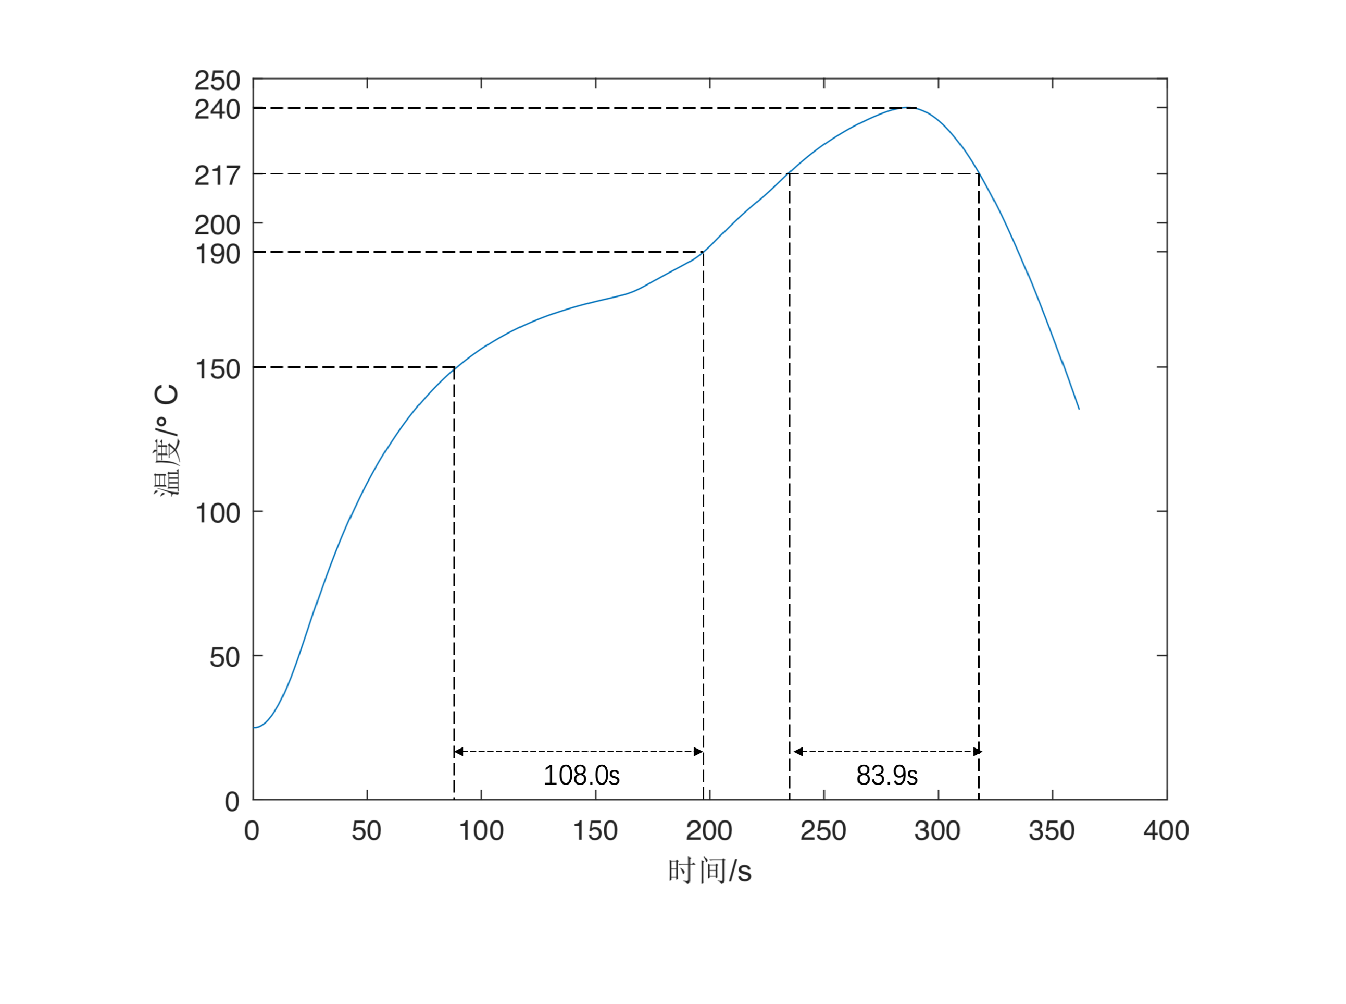
\includegraphics[scale=0.5]{Q2-2}
		\caption{最大速度对应炉温曲线}
	\end{figure}\par
	温度上升区斜率和下降区斜率最大值分别为2.39和2.28。由图可知,温度上升过程中在150$\sim$190°C的时间为108.0s,温度在超过217°C以上的时间为83.9s,且最大温度为240°C。均在制程界限内。
	\subsection{问题三的求解}
	问题三重点在于求取最优炉温曲线,其满足的前提为使超过217ºC到峰值温度所覆盖的面积最小,并需要给出最小值的具体值,同时要求温区的设定温度和传送带的过炉速度。\par
	\subsubsection{问题三模型的建立}
	首先确定目标函数为阴影面积最小值。其影响因素可从水平与竖直两方向看。水平方向代表焊接区域中心超过217°C时长,竖直方向代表最大峰值温度。现在就这两个影响因素给出目标函数计算方法。\par
	同问题一问题二,由于该区域解为离散型数值,把阴影区域沿时间$\tau$对应x轴分成宽度均匀的一个个小矩形,每个矩形内部均为连续型且宽度为$\varDelta\tau$,长度为$t_i\left(\tau\right)-217$。面积有如下表达:
	\begin{equation}
	\label{e7}
	\min S=\sum_{i}(t_i-217)\varDelta\tau\quad\quad 217\leqslant t_i\leqslant\max\left\{{t_i}\right\}
	\end{equation}\par
	约束条件使用第二问所设即可,有:
	\begin{equation}
	\label{e6}
	\text{s.t.}\begin{cases}
	-3\leqslant\dfrac{t_{i+1}-t_i}{\varDelta\tau}\leqslant 3\\[1em]
	60\leqslant\sum\limits_{\begin{smallmatrix}
		t_i\in[150,190],\\
		t_{i+1}\geqslant t_i
		\end{smallmatrix}} \varDelta\tau\leqslant 120\\[1em]
	40\leqslant\sum\limits_{t_i>217}\varDelta\tau\leqslant 90\\[1em]
	240\leqslant\max\limits_{i=1}^{n}\left\{t_i\right\}\leqslant 250\\
	\end{cases}
	\end{equation}\par
	\subsubsection{算法使用和模型求解}
	本问的模型为单目标优化模型。但由于变量较多,约束函数以及目标函数较复杂,这里使用遗传算法进行求解。其决策变量为四个大温区温度以及传送带运行速度。设向量$\boldsymbol x = (t_{I},t_{II},t_{III},t_{IV},v)$为决策变量向量,亦即种群个体,由题意,$\boldsymbol x$需要满足下式的边界条件:
	\begin{equation}
	\label{e5}
	(165,185,225,245,65) \leqslant \boldsymbol x \leqslant (185,205,245,265,100)
	\end{equation}\par
	其中的小于等于号表示向量元素在每一维上的关系。\par
	当决策变量$\boldsymbol x$给定后,就可以通过问题一建立的模型来求解得到相应的炉温曲线,进而结合式\ref{e6}来判断其是否满足制程界限要求。如果满足,其所对应的目标函数$S = S(\boldsymbol{x})$也就可以结合式\ref{e7}进行求解,即算法中所用目标函数。\par
	单目标遗传算法在本题中思路如下:以一个随机的初始种群开始迭代,在每一代中,对于可行解进行交叉和变异,根据约束条件选择较优可行解作为下一代种群,在迭代一定次数后终止算法,得到最优可行解。具体算法过程不再赘述,使用Matlab内置的优化工具箱中的ga函数进行求解。在本问题中设置种群大小为100,迭代500代。\par
	另外,在本问题以及问题四中,需要大量求解不同边界温度下的$t_f$值,而这在之前的模型中是需要对微分方程求数值解才能得到。这一过程实际是非常耗时的。注意到由于回焊炉的宽度$d$不大,可以用边界温度代替泛炉内加热区温度$t_f$,这一点的合理性可以从图3中看出。\par
	经过遗传算法迭代,产生最小阴影面积S为461.14$^\circ$C$\cdot$s,对应的决策变量取值如下表2:
	\begin{table}[h]
		\centering
		\caption{问题三变量取值表}
		\begin{tabular}{ccccc }
			\toprule
			$t_{I}$ & $t_{II}$ & $t_{III}$ & $t_{IV}$ & $v$\\ \midrule
			179.59$^\circ$C & 203.12$^\circ$C & 244.49$^\circ$C & 265.00$^\circ$C & 99.98cm/min\\
			\bottomrule 
		\end{tabular}
		\label{t1}
	\end{table}\par	
	对应的炉温曲线如图10所示:\par
	\begin{figure}[H]
		\centering
		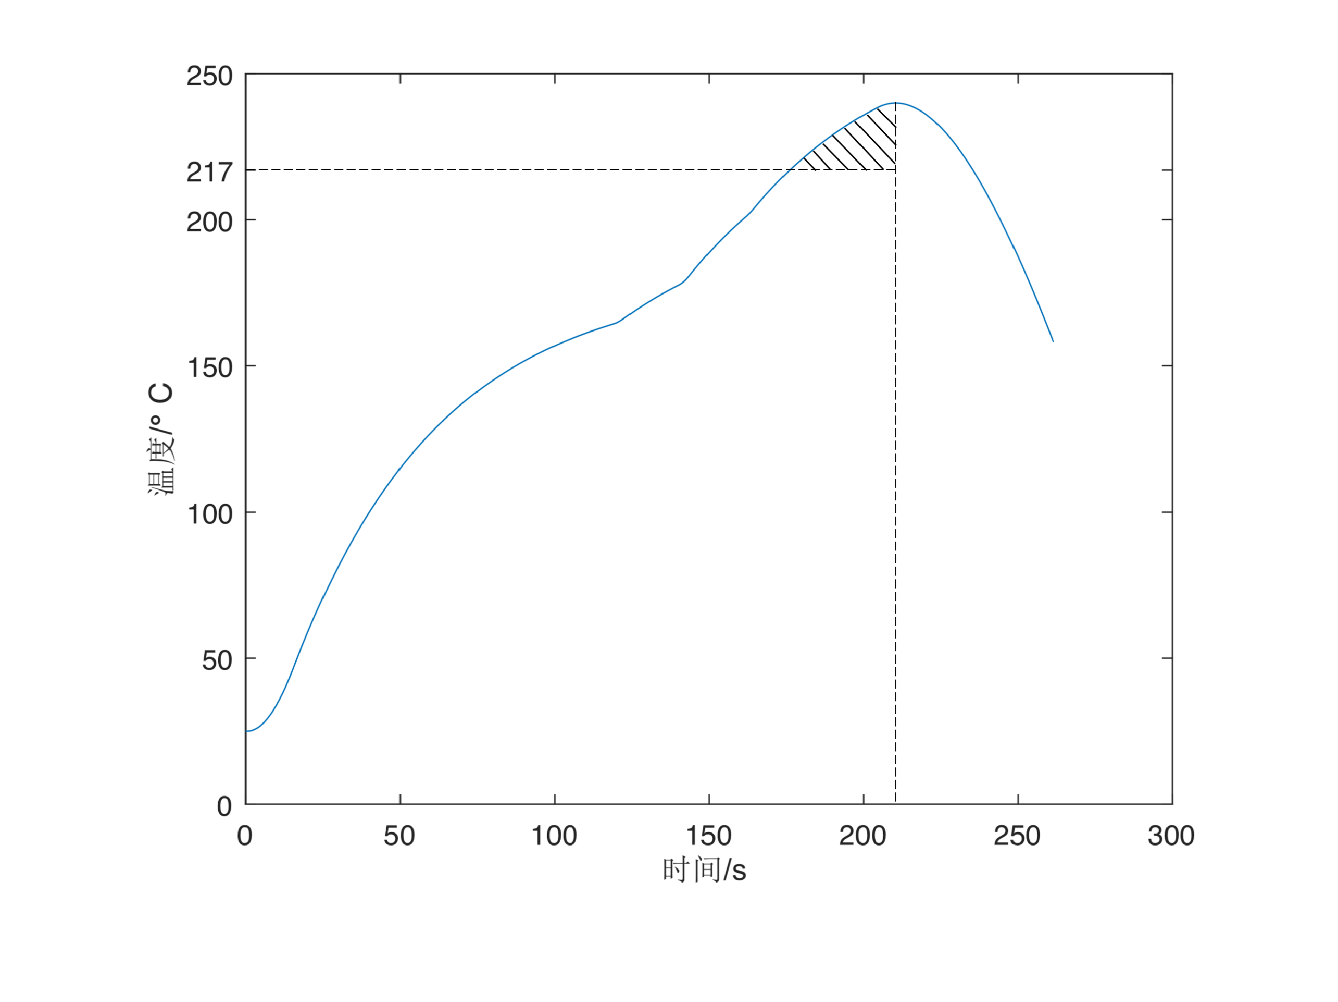
\includegraphics[scale=0.5]{Q3-shadow}
		\caption{最小阴影面积与炉温曲线示意图}
	\end{figure}\par
	\subsubsection{模型制约界限验证}
	如图10,温度上升区斜率和下降区斜率最大值分别为2.80和2.74。温度上升过程中在150$\sim$190°C的时间为63.63s,温度在超过217°C以上的时间为59.27s,且最大温度为240°C。均在制程界限内。由此可知,使最大温度尽可能低,过温区速度尽可能快(时间尽可能短)都是达到最低面积的必要条件。\par
	\subsection{问题四的求解}
	问题四希望在满足问题三最小阴影面积的基础上,使以峰值温度为中心线两侧超过217ºC的炉温曲线形状尽量对称。求取该约束下最优炉温曲线,各温区设定的温度和传送带过炉速度。\par
	\subsubsection{目标函数和制约条件确定}
	与第三问类似,决策变量为四个大温区温度和传送带速度,仍用向量$\boldsymbol{x}$表示,约束条件同式\ref{e6}。\par
	关于目标函数,我们仍有如式\ref{e7}的目标函数$S = S(\boldsymbol{x})$。另外,对于问题四中要求的尽可能使曲线对称,我们采用如下的指标衡量其对称度:
	\begin{equation}
	E = \sqrt{\frac{\sum\limits_{i}\left(t_{m+i} - t_{m-i}\right)^2}{\sum\limits_{i} 1}},\quad\quad t_{m-i},t_{m+i}>217
	\end{equation}\par
	其中$t_m = \max\left\{t_i\right\}$为炉温曲线的最高点。上式从直观上可以理解为,取最高点两侧对称的取样点之间的差距平均值来衡量对称度。这样定义的$E$,实际上也可以通过炉温曲线$t$间接的表示成$E = E(\boldsymbol{x})$的形式。综合上述说明,问题四的优化模型如下:
	\begin{equation}
	\begin{cases}
	\min &S=\sum\limits_{i}(t_i-217)\varDelta\tau,\quad\quad 217\leqslant t_i\leqslant\max\left\{{t_i}\right\}\\[1em]
	\min &E =\sqrt{\frac{\sum\limits_{i}\left(t_{m+i} - t_{m-i}\right)^2}{\sum\limits_{i} 1}},\quad\quad t_{m-i},t_{m+i}>217\\[1em]
	\text{s.t.}&-3\leqslant\dfrac{t_{i+1}-t_i}{\varDelta\tau}\leqslant 3\\[1em]
	&60\leqslant\sum\limits_{\begin{smallmatrix}
		t_i\in[150,190],\\
		t_{i+1}\geqslant t_i
		\end{smallmatrix}} \varDelta\tau\leqslant 120\\[1em]
	&40\leqslant\sum\limits_{t_i>217}\varDelta\tau\leqslant 90\\[1em]
	&240\leqslant\max\limits_{i=1}^{n}\left\{t_i\right\}\leqslant 250
	\end{cases}
	\end{equation}\par
	其中的$t_i$由$\boldsymbol{x}$确定,而$\boldsymbol{x}$也要满足式\ref{e5}的约束条件。
	\subsubsection{多目标优化模型的求解}
	可以注意到,问题四是一个多目标的优化模型。因此本文采用多目标遗传算法NSGA-II进行求解。同样,Matlab中优化工具箱自带gamultiobj函数,拥有可以实现这一算法的功能。设置初始种群大小为300,迭代1000次,最终得到图11所示的Pareto前沿图,同时生成了Q4.xls文件储存各点的信息,以供进一步选择。
	\begin{figure}[H]
		\centering
		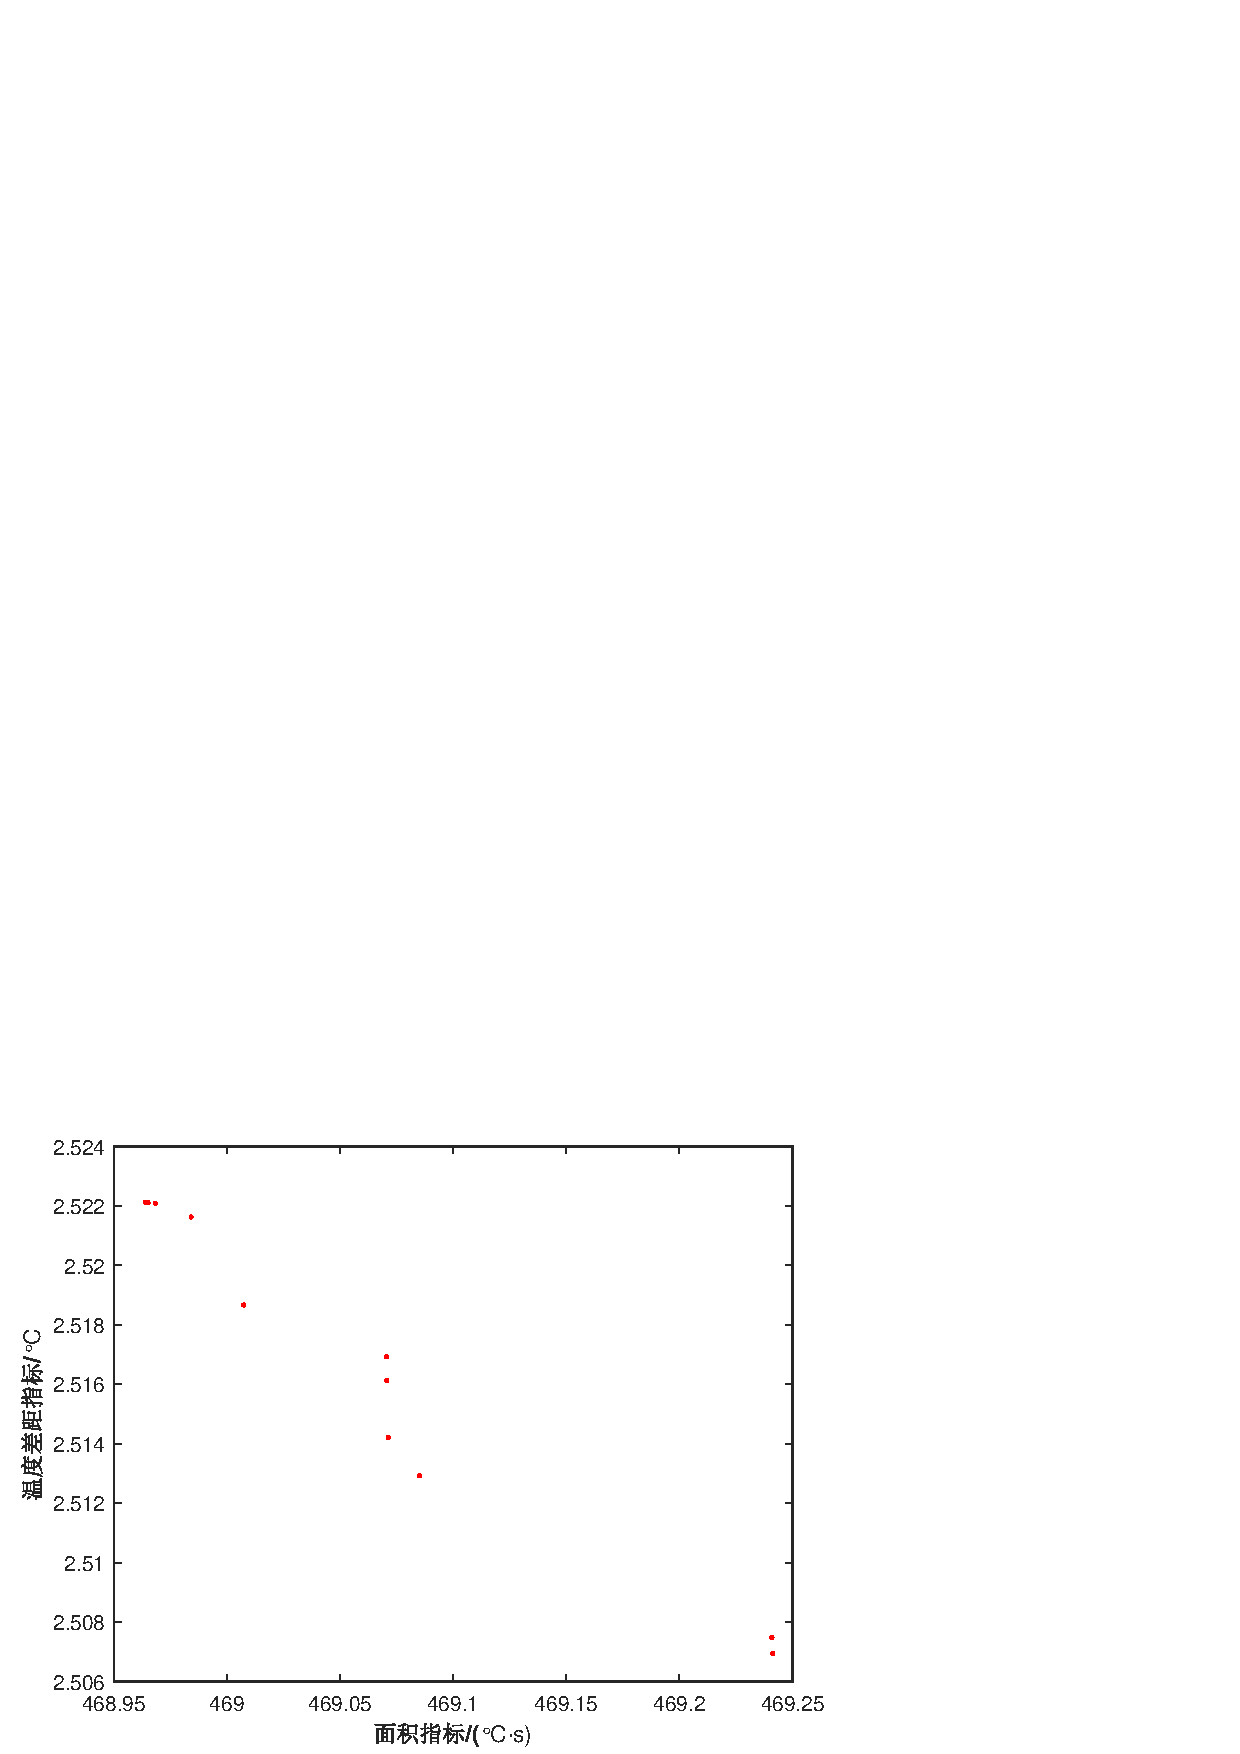
\includegraphics[scale=0.6]{Q4pareto}
		\caption{问题四结果的Pareto前沿图}
	\end{figure}\par
	从图中可以看出,最优的对称度指标稳定在2.5左右,而面积指标稳定在468左右。本文选择图上最右下方的点为本问题的最终结果,而在实际生产中可以根据实际需要选择不同的Pareto前沿点分析。这一点对应的$\boldsymbol{x}$取值如表3:\par\par
	\begin{table}[h]
		\centering
		\caption{问题四变量取值表}
		\begin{tabular}{ccccc}
		\toprule
		$t_{I}$ & $t_{II}$ & $t_{III}$ & $t_{IV}$ & $v$\\ \midrule
		167.72$^\circ$C & 191.99$^\circ$C & 228.72$^\circ$C & 265.00$^\circ$C & 88.16cm/min\\
		\bottomrule 
		\end{tabular}
		\label{t2}
	\end{table}\par
	画出的炉温曲线如图12所示。
	\begin{figure}[H]
		\centering
		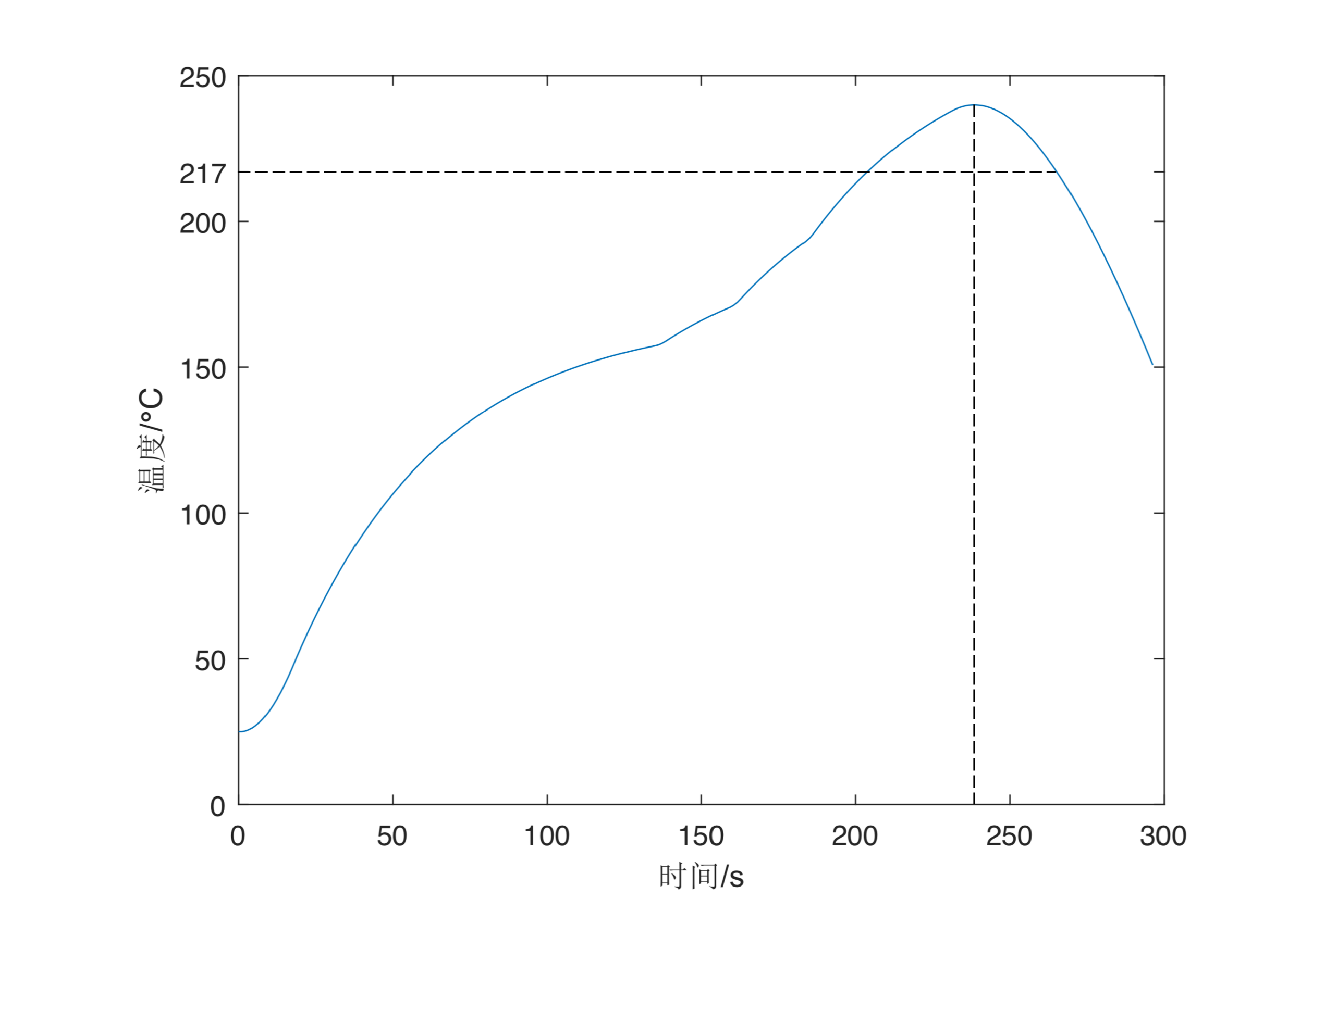
\includegraphics[scale=0.48]{Q4-2}
		\caption{问题四结果炉温曲线图}
	\end{figure}\par
	此时超过217$^\circ$C区域面积为469.24$^\circ$C$\cdot$s,两侧对称位置的温度平均差距为2.51$^\circ$C。\par
	同样本文对制程界限做检测,如上图,温度上升区斜率和下降区斜率最大值分别为2.54和2.59。温度上升过程中在150$\sim$190°C的时间为70.44s,温度在超过217°C以上的时间为61.42s,且最大温度为240.0°C。均在制程界限内。\par
	\section{模型的灵敏度分析及误差分析}
	分析对模型精确性的影响因素,主要有以下两点。\par
	1.模型使用的是结合附件拟合的时间常数$\tau_c$,可能拟合的结果不够精确。同时,由于$\tau_c$本身与焊接原件和周围空气的相对速度可能有关,因此在锅炉速度变化的前提下其值有可能发生改变。因此,有必要进行炉温曲线对于时间常数的灵敏度分析。\par
	2.三四问的模型均使用回焊炉的边界温度代替其中心的实际温度,这样也可能带来误差。因此有必要对其进行分析。\par
	\subsection{对时间常数$\tau_c$进行的灵敏度分析}
	取$t_c=$43,48,53三个不同的数值,在附件所对应的温度、速度情况下,做出对应的炉温曲线图如图13。
	\begin{figure}[H]
		\centering
		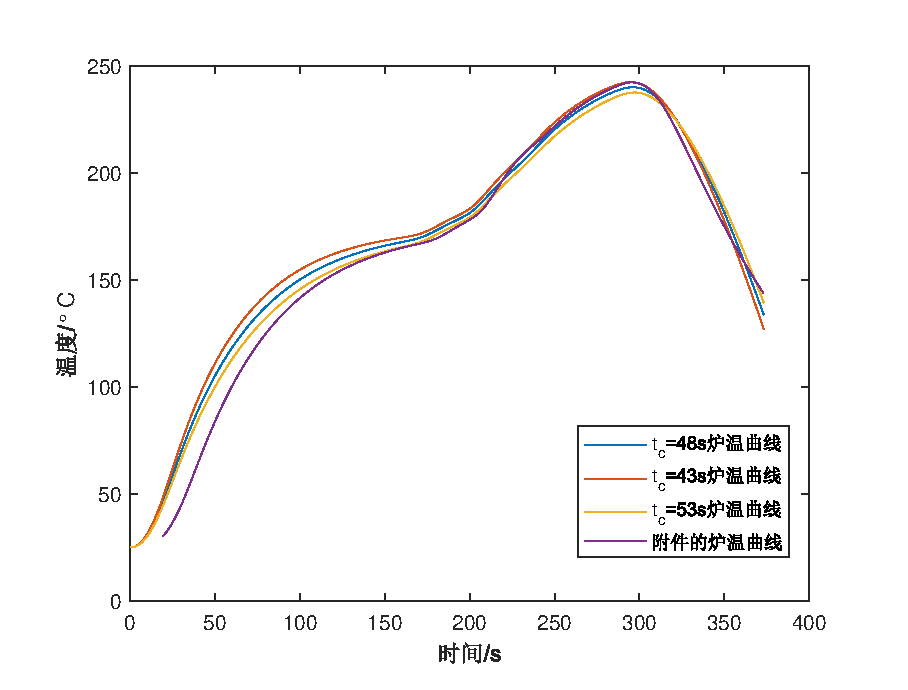
\includegraphics[scale=0.7]{ex_tc}
		\caption{不同$\tau_c$下的炉温曲线}
	\end{figure}\par
	可以看出,在200s后四条曲线基本重合,误差非常小。而在初始的200s内,三个不同$\tau_c$之间的差距也并不大。因此,可以认为炉温曲线对于时间常数的灵敏度并不高,$\tau_c$的值在$\pm10s$内变化时曲线误差不大。
	\subsection{对近似炉心温度$t_f$的误差分析}
	仍在附件对应的条件下进行误差分析。原仿真的结果图与用边界温度代替炉心温度后的仿真结果图如图14:
	\begin{figure}[H]
		\centering
		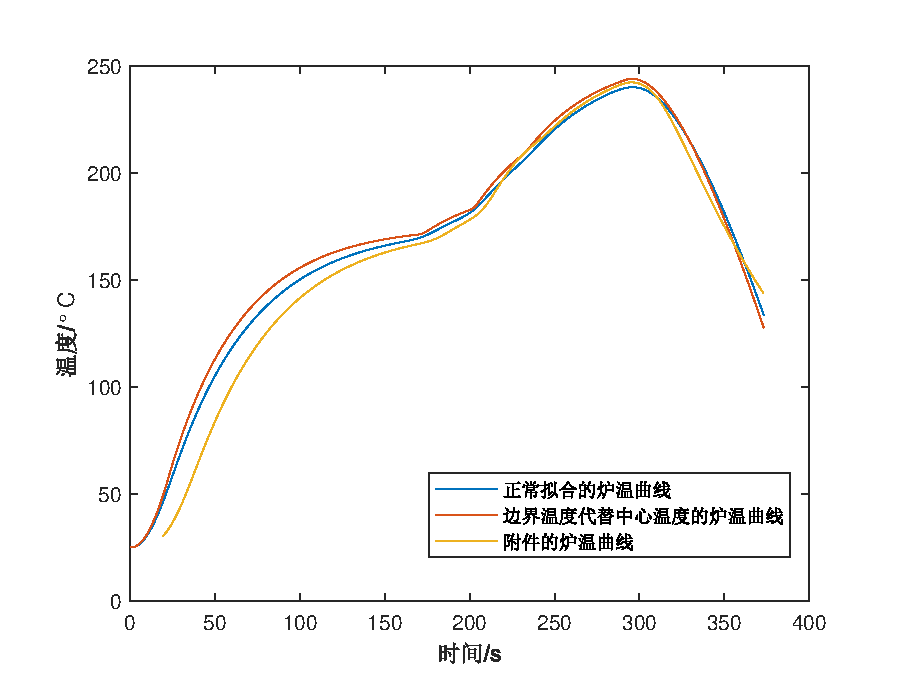
\includegraphics[scale=0.7]{ex_2}
		\caption{不同近似方法温度对比图}
	\end{figure}\par
	其结果与上图类似,在200s后的部分几乎没有误差,而在200s前的误差也在可接受的范围内。因此,为了提高运行速度而做出的这一代替是可行的。
	%参考文献
	\begin{thebibliography}{9}%宽度9
		\bibitem{ref1}蔡海涛, 李威, 王浩. 回流焊接温度曲线控制研究[J]. 微处理机, 2008, 29(005):24-26.
		\bibitem{ref2}赵镇南. 传热学 [M]. 第三版, 北京:高等教育出版社,(2019)  
		\bibitem{ref3}华东英,李详贵. 微分方程的数值解法与程序实现 [M]. 第三版, 北京:电子工业出版社,(2016)  
	\end{thebibliography}
	
	\newpage
	\begin{center}
		\large\textbf{附录}\\\par
	\end{center}
	\centering\noindent\normalsize\textbf{支撑材料目录}
	\begin{table}[h]
	\centering
	\begin{tabular}{cc}
		\toprule
		文件 & 说明\\  \midrule

Q0.m & 求解$\tau_c$程序\\
Q1.m & 问题一程序\\
Q2.m & 问题二程序\\
Q3.m & 问题三程序\\
Q4.m & 问题四程序\\
ex.m & 灵敏度分析程序\\
Q1-1.eps & 图片\\
Q1-2.eps& 图片\\
Q1-3.eps& 图片\\
Q1-4.eps& 图片\\
Q1-5.eps& 图片\\
Q1-6.eps& 图片\\
Q1-edge.eps& 图片\\
Q2-1.eps& 图片\\
Q2-2.eps& 图片\\
Q3-shadow.eps& 图片\\
Q4-2.eps& 图片\\
Q4pareto.eps& 图片\\
ex$\_$2.eps& 图片\\
ex$\_$tc.eps& 图片\\
result.csv&问题一结果\\
Q4.xlsx&问题四中间过程\\
		\bottomrule 
	\end{tabular}
\end{table}\par




	\noindent\normalsize\textbf{求解$\tau_c$}
	\begin{lstlisting}[language=matlab]
xls = xlsread('附件.xlsx','A2:B710');
tim = xls(:,1);
t = xls(:,2);
v = 7/6*0.01;
len = 435.5e-2;
% plot(tim,t);
KK = 273.15;

ll = 15e-2;    % 宽度
h = 0.5 / 100;
k = 0.1 / 100;
x = 0:h:(len);
y = 0:k:(ll);
%% 炉心温度
temp = zeros(1,length(x));
for i = 1:length(x)
temp(i) = get_t(x(i));
end
plot(x*100,temp)
hold on
interation = 50000;
n = size(x,2);
m = size(y,2);
z_p = ones(n,m) * 0;
z_c = ones(n,m) * 0;
A = [h^2,h^2,k^2,k^2];
Eps = 1e-3;
w = 1.7;
for int = 1:interation
for j = 1:m
z_c(1,j) = 25 + KK;
z_c(n,j) = 25 + KK;
end
for i = 1:n
z_c(i,m) = get_t(x(i)) + KK;
z_c(i,1) = get_t(x(i)) + KK;
end
for i = 2:n-1
for j = 2:m-1
z_c(i,j) = (1-w)*z_p(i,j) + w*(dot(A,[z_c(i,j-1),z_p(i,j+1),z_c(i-1,j),z_p(i+1,j)]))/2/(h^2+k^2);
end
end
err = sqrt(sum((z_p - z_c).^2)/length(z_c));
if(err<Eps)
break;
end
z_p = z_c;
end
z_p = z_p - KK;
% [x,y]=meshgrid(x,y);
% mesh(x',y',z_p);
tt = ll/2 / k;
xlswrite('z0.xls',z_p(:,tt));
plot(x*100,z_p(:,tt))
legend('边界线温度','中心线温度')
xlabel('位置/cm')
ylabel('温度/\circC')
%% 大范围搜索t_c
step = 0.01;
t_e = xlsread('z0.xls') + KK;
hold on
ti = 0:step:(len/v);     % 时间
t_c = 1:1:100;
t_0 = zeros(1,length(ti));
err = zeros(1,length(t_c));
for kkkk = 1:length(t_c)
t_0(1) = 25 + KK;
for i = 2:length(ti)
t_f = t_e(get_t2(ti(i),v,x));
t_0(i) = t_0(i-1) + step * (t_0(i-1) - t_f) / (-t_c(kkkk));
end
ccc = 1;
err(kkkk) = 0;
for i = 1:length(ti)
if(ccc>length(t))
break;
end
if(abs(ti(i) - tim(ccc))<step/2)
err(kkkk) = err(kkkk) + (t_0(i)-KK - t(ccc))^2;
ccc = ccc + 1;
end
end
err(kkkk) = err(kkkk) / length(t);
err(kkkk) = sqrt(err(kkkk));
end
plot(t_c,err)
xlabel('时间常数t_c/s');
ylabel('平均误差/\circC');
%% 三分法
l = 0.01;r = 100;
step = 0.01;
t_e = xlsread('z0.xls') + KK;
ti = 0:step:(len/v);     % 时间
t_0 = zeros(1,length(ti));
while(r-l>=1e-6)
m1 = (2*l+r)/3;
m2 = (l+2*r)/3;
% e1
t_0(1) = 25 + KK;
for i = 2:length(ti)
t_f = t_e(get_t2(ti(i),v,x));
t_0(i) = t_0(i-1) + step * (t_0(i-1) - t_f) / (-m1);
end
ccc = 1;
e1 = 0;
for i = 1:length(ti)
if(ccc>length(t))
break;
end
if(abs(ti(i) - tim(ccc))<step/2)
e1 = e1 + (t_0(i)-KK - t(ccc))^2;
ccc = ccc + 1;
end
end
e1 = e1 / length(t);
e1 = sqrt(e1);
re = check(t_0,ti);
if(re(5)-KK<240) 
e1 = 1e7;
end
% e2
t_0(1) = 25 + KK;
for i = 2:length(ti)
t_f = t_e(get_t2(ti(i),v,x));
t_0(i) = t_0(i-1) + step * (t_0(i-1) - t_f) / (-m2);
end
ccc = 1;
e2 = 0;
for i = 1:length(ti)
if(ccc>length(t))
break;
end
if(abs(ti(i) - tim(ccc))<step/2)
e2 = e2 + (t_0(i)-KK - t(ccc))^2;
ccc = ccc + 1;
end
end
e2 = e2 / length(t);
e2 = sqrt(e2);
re = check(t_0,ti);
if(re(5)-KK<240) 
e2 = 1e7;
end
if(e1>e2)
l = m1;
else
r = m2;
end
end
l
r
e1
e2
%% 最优t_c = 47.9567画图(err = 9.55)
tc_real = 47.9567;
ti = 0:step:(len/v);     % 时间
t_0 = zeros(1,length(ti));
t_0(1) = 25 + KK;
for i = 2:length(ti)
t_f = t_e(get_t2(ti(i),v,x));
t_0(i) = t_0(i-1) + step * (t_0(i-1) - t_f) / (-tc_real);
end
plot(ti,t_0-KK);
hold on
plot(tim,t);
legend('t_c=47.9567s炉温曲线','附件的炉温曲线');
xlabel('时间/s')
ylabel('温度/\circ C')

%% 边界温度分布函数
function temp = get_t(x)
to = 25;
t1 = 175;
t2 = 195;
t3 = 235;
t4 = 255;
x = x * 100;
len = 435.5;
if(x<=25)
temp = to + (t1 - to)/25 * x;
elseif(x<=25 + 30.5*5 + 5*4)
temp = t1;
elseif(x<=25 + 30.5*5 + 5*5)
temp = t1 + (t2-t1)/5 * (x - (25 + 30.5*5 + 5*4));
elseif(x<=25 + 30.5*6 + 5*5)
temp = t2;
elseif(x<=25 + 30.5*6 + 5*6)
temp = t2 + (t3-t2)/5 * (x - (25 + 30.5*6 + 5*5));
elseif(x<=25 + 30.5*7 + 5*6)
temp = t3;
elseif(x<=25 + 30.5*7 + 5*7)
temp = t3 + (t4-t3)/5 * (x - (25 + 30.5*7 + 5*6));
elseif(x<=25 + 30.5*9 + 5*8)
temp = t4;
else
temp = (len - x)/(len - (25 + 30.5*9 + 5*8))*(t4 - to) + to;
end
end

%% 时间对应环境温度
function idx = get_t2(tim,v,x)
l = 1;r = length(x);
while(r-l>=5)
mid = floor((l+r)/2);
if(tim*v<x(mid))
r = mid;
else
l = mid;
end
end
for i = l:r
if(tim*v>=x(i))
idx = l;
break;
end
end
end
%% 炉温曲线检验
function res = check(t, ti)
delta = ti(2) - ti(1);
res = [0,1e9,0,0,0];
for i = 2:length(t)
if(i>1)
res(1) = max(res(1),(t(i)-t(i-1))/delta);
res(2) = min(res(2),(t(i)-t(i-1))/delta);
if(t(i)-t(i-1)>=0 && t(i)<=190 && t(i)>=150)
res(3) = res(3) + delta;
end
end
if(t(i)>217)
res(4) = res(4) + delta;
end
end
res(5) = max(t);
end
	\end{lstlisting}\par
	\noindent\normalsize\textbf{Q1}
	\begin{lstlisting}[language=matlab]
v = 78/60*0.01;
len = 435.5e-2;
KK = 273.15;

ll = 15e-2;    % 宽度
h = 0.5 / 100;
k = 0.1 / 100;
x = 0:h:(len);
y = 0:k:(ll);
%% 炉心温度
interation = 50000;
n = size(x,2);
m = size(y,2);
z_p = ones(n,m) * 0;
z_c = ones(n,m) * 0;
A = [h^2,h^2,k^2,k^2];
Eps = 1e-3;
w = 1.7;
for int = 1:interation
for j = 1:m
z_c(1,j) = 25 + KK;
z_c(n,j) = 25 + KK;
end
for i = 1:n
z_c(i,m) = get_t(x(i)) + KK;
z_c(i,1) = get_t(x(i)) + KK;
end
for i = 2:n-1
for j = 2:m-1
z_c(i,j) = (1-w)*z_p(i,j) + w*(dot(A,[z_c(i,j-1),z_p(i,j+1),z_c(i-1,j),z_p(i+1,j)]))/2/(h^2+k^2);
end
end
err = abs(z_p - z_c);
if(all(err<Eps))
break;
end
z_p = z_c;
end
z_p = z_p - KK;
tt = ll/2 / k;
xlswrite('z1.xls',z_p(:,tt));
%% 炉温曲线
tc_real = 47.9567;
step = 0.01;
t_e = xlsread('z1.xls') + KK;
ti = 0:step:(len/v);     % 时间
t_0 = zeros(1,length(ti));
t_0(1) = 25 + KK;
for i = 2:length(ti)
t_f = t_e(get_t2(ti(i),v,x));
t_0(i) = t_0(i-1)+step*(t_0(i-1)-t_f-2)/(-tc_real);
end
plot(ti,t_0-KK);
xlabel('时间/s')
ylabel('温度/\circ C')
res_time = [];
res_temp = [];
for i = 1:length(t_0)
if(mod(i,50)==1)
res_time = [res_time, ti(i)];
res_temp = [res_temp, t_0(i)];
end
end
xlswrite('result.xlsx',[res_time;res_temp-KK]');
ch = check(t_0-KK,ti);
t_0 = t_0 - KK;
ch(1)
ch(2)
ch(3)
ch(4)
ch(5)
%% 炉温曲线检验
function res = check(t, ti)
delta = ti(2) - ti(1);
res = [0,1e9,0,0,0];
for i = 2:length(t)
if(i>1)
res(1) = max(res(1),(t(i)-t(i-1))/delta);
res(2) = min(res(2),(t(i)-t(i-1))/delta);
if(t(i)-t(i-1)>=0 && t(i)<=190 && t(i)>=150)
res(3) = res(3) + delta;
end
end
if(t(i)>217)
res(4) = res(4) + delta;
end
end
res(5) = max(t);
end
%% 边界温度分布函数
function temp = get_t(x)
to = 25;
t1 = 173;
t2 = 198;
t3 = 230;
t4 = 257;
x = x * 100;
len = 435.5;
if(x<=25)
temp = to + (t1 - to)/25 * x;
elseif(x<=25 + 30.5*5 + 5*4)
temp = t1;
elseif(x<=25 + 30.5*5 + 5*5)
temp = t1 + (t2-t1)/5 * (x - (25 + 30.5*5 + 5*4));
elseif(x<=25 + 30.5*6 + 5*5)
temp = t2;
elseif(x<=25 + 30.5*6 + 5*6)
temp = t2 + (t3-t2)/5 * (x - (25 + 30.5*6 + 5*5));
elseif(x<=25 + 30.5*7 + 5*6)
temp = t3;
elseif(x<=25 + 30.5*7 + 5*7)
temp = t3 + (t4-t3)/5 * (x - (25 + 30.5*7 + 5*6));
elseif(x<=25 + 30.5*9 + 5*8)
temp = t4;
else
temp = (len - x)/(len - (25 + 30.5*9 + 5*8))*(t4 - to) + to;
end
end

%% 时间对应温度
function idx = get_t2(tim,v,x)
l = 1;r = length(x);
while(r-l>=5)
mid = floor((l+r)/2);
if(tim*v<x(mid))
r = mid;
else
l = mid;
end
end
for i = l:r
if(tim*v>=x(i))
idx = l;
break;
end
end
end
	\end{lstlisting}
	\noindent\normalsize\textbf{Q2}
	\begin{lstlisting}[language=matlab]
v = (65:100)/60/100;
len = 435.5e-2;
KK = 273.15;

ll = 15e-2;    % 宽度
h = 0.5 / 100;
k = 0.1 / 100;
x = 0:h:(len);
y = 0:k:(ll);
%% 炉心温度
interation = 50000;
n = size(x,2);
m = size(y,2);
z_p = ones(n,m) * 0;
z_c = ones(n,m) * 0;
A = [h^2,h^2,k^2,k^2];
Eps = 1e-3;
w = 1.7;
for int = 1:interation
for j = 1:m
z_c(1,j) = 25 + KK;
z_c(n,j) = 25 + KK;
end
for i = 1:n
z_c(i,m) = get_t(x(i)) + KK;
z_c(i,1) = get_t(x(i)) + KK;
end
for i = 2:n-1
for j = 2:m-1
z_c(i,j) = (1-w)*z_p(i,j) + w*(dot(A,[z_c(i,j-1),z_p(i,j+1),z_c(i-1,j),z_p(i+1,j)]))/2/(h^2+k^2);
end
end
err = abs(z_p - z_c);
if(all(err<Eps))
break;
end
z_p = z_c;
end
z_p = z_p - KK;
tt = ll/2 / k;
xlswrite('z2.xls',z_p(:,tt));
%% 大步长画图
tc_real = 47.9567;
step = 0.01;
t_e = xlsread('z2.xls') + KK;
ch = zeros(5,length(v));
for ttt = 1:length(v)
ti = 0:step:(len/v(ttt));     % 时间
t_0 = zeros(1,length(ti));
t_0(1) = 25 + KK;
for i = 2:length(ti)
t_f = t_e(get_t2(ti(i),v(ttt),x));
t_0(i) = t_0(i-1) + step * (t_0(i-1) - t_f) / (-tc_real);
end
ch(:,ttt) = check(t_0-KK,ti);
end
plot(v*100*60,ch(1,:)*10);
hold on
plot(v*100*60,ch(2,:)*10);
hold on
plot(v*100*60,ch(3,:));
hold on
plot(v*100*60,ch(4,:));
hold on
plot(v*100*60,ch(5,:));
legend('温度上升斜率最高值*10','温度下降斜率最低值*10','上升过程中在150\circC-190\circC的时间','温度大于217?C的时间','峰值温度');
xlabel('速度/(cm/min)')
ylabel('制程界限')
%% 搜索最大可行v
v = (70:0.01:75)/60/100;
tc_real = 47.9567;
step = 0.01;
t_e = xlsread('z2.xls') + KK;
ch = zeros(5,length(v));
for ttt = 1:length(v)
ti = 0:step:(len/v(ttt));     % 时间
t_0 = zeros(1,length(ti));
t_0(1) = 25 + KK;
for i = 2:length(ti)
t_f = t_e(get_t2(ti(i),v(ttt),x));
t_0(i) = t_0(i-1) + step * (t_0(i-1) - t_f) / (-tc_real);
end
ch(:,ttt) = check(t_0-KK,ti);
end
res = 0;
for i = length(v):-1:1
if(ch(1,i)<=3 && ch(2,i)>=-3 && ch(3,i)>=60 && ch(3,i)<=120 &&...
ch(4,i)>=40 && ch(4,i)<=90 && ch(5,i)>=240 && ch(5,i)<=250)
res = v(i);
break
end
end
res*60*100
%% 最优v=72.25画图
v = 72.25/60/100;
ti = 0:step:(len/v);     % 时间
t_0 = zeros(1,length(ti));
t_0(1) = 25 + KK;
for i = 2:length(ti)
t_f = t_e(get_t2(ti(i),v,x));
t_0(i) = t_0(i-1) + step * (t_0(i-1) - t_f) / (-tc_real);
end
plot(ti,t_0-KK);
xlabel('时间/s')
ylabel('温度/\circ C')
ch = check(t_0-KK,ti)


%% 炉温曲线检验
function res = check(t, ti)
delta = ti(2) - ti(1);
res = [0,1e9,0,0,0];
for i = 2:length(t)
if(i>1)
res(1) = max(res(1),(t(i)-t(i-1))/delta);
res(2) = min(res(2),(t(i)-t(i-1))/delta);
if(t(i)-t(i-1)>=0 && t(i)<=190 && t(i)>=150)
res(3) = res(3) + delta;
end
end
if(t(i)>217)
res(4) = res(4) + delta;
end
end
res(5) = max(t);
end
%% 边界温度分布函数
function temp = get_t(x)
to = 25;
t1 = 182;
t2 = 203;
t3 = 237;
t4 = 254;
x = x * 100;
len = 435.5;
if(x<=25)
temp = to + (t1 - to)/25 * x;
elseif(x<=25 + 30.5*5 + 5*4)
temp = t1;
elseif(x<=25 + 30.5*5 + 5*5)
temp = t1 + (t2-t1)/5 * (x - (25 + 30.5*5 + 5*4));
elseif(x<=25 + 30.5*6 + 5*5)
temp = t2;
elseif(x<=25 + 30.5*6 + 5*6)
temp = t2 + (t3-t2)/5 * (x - (25 + 30.5*6 + 5*5));
elseif(x<=25 + 30.5*7 + 5*6)
temp = t3;
elseif(x<=25 + 30.5*7 + 5*7)
temp = t3 + (t4-t3)/5 * (x - (25 + 30.5*7 + 5*6));
elseif(x<=25 + 30.5*9 + 5*8)
temp = t4;
else
temp = (len - x)/(len - (25 + 30.5*9 + 5*8))*(t4 - to) + to;
end
end

%% 时间对应温度
function idx = get_t2(tim,v,x)
l = 1;r = length(x);
while(r-l>=5)
mid = floor((l+r)/2);
if(tim*v<x(mid))
r = mid;
else
l = mid;
end
end
for i = l:r
if(tim*v>=x(i))
idx = l;
break;
end
end
end
\end{lstlisting}
	\noindent\normalsize\textbf{Q3}
	\begin{lstlisting}[language=matlab]
x0 = [175,195,235,255,80];
lb = [165,185,225,245,65];
ub = [185,205,245,265,100];

options=optimoptions('ga','PopulationSize',100,'MaxGenerations',500);
[x,fval,exitflag,output] = ga(@(x)fun(x),5,[],[],[],[],lb,ub,@(x)nonlcon(x),options)
t1 = x(1);
t2 = x(2);
t3 = x(3);
t4 = x(4);
v = x(5)/100/60;
len = 435.5e-2;
KK = 273.15;
h = 0.5 / 100;
x = 0:h:(len);
% 炉心温度
t_e = zeros(1,length(x));
for i = 1:length(t_e)
t_e(i) = get_t(t1,t2,t3,t4,x(i)) + KK;
end
% 求解炉温曲线
tc_real = 47.9567;
step = 0.01;
ti = 0:step:(len/v);     % 时间
t_0 = zeros(1,length(ti));
t_0(1) = 25 + KK;
for i = 2:length(ti)
t_f = t_e(get_t2(ti(i),v,x));
t_0(i) = t_0(i-1) + step * (t_0(i-1) - t_f) / (-tc_real);
end
t_0 = t_0 - KK;
plot(ti,t_0);
check(t_0,ti)


% fun(ub)
%% 
function area = fun(X)
t1 = X(1);
t2 = X(2);
t3 = X(3);
t4 = X(4);
v = X(5)/100/60;
len = 435.5e-2;
KK = 273.15;
h = 0.5 / 100;
x = 0:h:(len);
% 炉心温度
t_e = zeros(1,length(x));
for i = 1:length(t_e)
t_e(i) = get_t(t1,t2,t3,t4,x(i)) + KK;
end
% 求解炉温曲线
tc_real = 47.9567;
step = 0.01;
ti = 0:step:(len/v);     % 时间
t_0 = zeros(1,length(ti));
t_0(1) = 25 + KK;
for i = 2:length(ti)
t_f = t_e(get_t2(ti(i),v,x));
t_0(i) = t_0(i-1) + step * (t_0(i-1) - t_f) / (-tc_real);
end
t_0 = t_0 - KK;
[~,idx] = max(t_0);
area = 0;
for i = 1:idx
if(t_0(i)>217)
area = area + (t_0(i)-217) * step;
end
end
end
%% a
function [c,ceq] = nonlcon(X)
t1 = X(1);
t2 = X(2);
t3 = X(3);
t4 = X(4);
v = X(5)/100/60;
len = 435.5e-2;
KK = 273.15;
h = 0.5 / 100;
x = 0:h:(len);
% 炉心温度
t_e = zeros(1,length(x));
for i = 1:length(t_e)
t_e(i) = get_t(t1,t2,t3,t4,x(i)) + KK;
end
% 求解炉温曲线
tc_real = 47.9567;
step = 0.01;
ti = 0:step:(len/v);     % 时间
t_0 = zeros(1,length(ti));
t_0(1) = 25 + KK;
for i = 2:length(ti)
t_f = t_e(get_t2(ti(i),v,x));
t_0(i) = t_0(i-1) + step * (t_0(i-1) - t_f) / (-tc_real);
end
ch = check(t_0-KK,ti);
c = [ch(1) - 3;
- 3 - ch(2);
ch(3) - 120;
60 - ch(3);
ch(4) - 90;
40 - ch(4);
ch(5) - 250;
240 - ch(5)];
ceq = [];
end
%% 炉温曲线检验
function res = check(t, ti)
delta = ti(2) - ti(1);
res = [0,1e9,0,0,0];
for i = 2:length(t)
if(i>1)
res(1) = max(res(1),(t(i)-t(i-1))/delta);
res(2) = min(res(2),(t(i)-t(i-1))/delta);
if(t(i)-t(i-1)>=0 && t(i)<=190 && t(i)>=150)
res(3) = res(3) + delta;
end
end
if(t(i)>217)
res(4) = res(4) + delta;
end
end
res(5) = max(t);
end
%% 边界温度分布函数
function temp = get_t(t1,t2,t3,t4,x)
to = 25;
x = x * 100;
len = 435.5;
if(x<=25)
temp = to + (t1 - to)/25 * x;
elseif(x<=25 + 30.5*5 + 5*4)
temp = t1;
elseif(x<=25 + 30.5*5 + 5*5)
temp = t1 + (t2-t1)/5 * (x - (25 + 30.5*5 + 5*4));
elseif(x<=25 + 30.5*6 + 5*5)
temp = t2;
elseif(x<=25 + 30.5*6 + 5*6)
temp = t2 + (t3-t2)/5 * (x - (25 + 30.5*6 + 5*5));
elseif(x<=25 + 30.5*7 + 5*6)
temp = t3;
elseif(x<=25 + 30.5*7 + 5*7)
temp = t3 + (t4-t3)/5 * (x - (25 + 30.5*7 + 5*6));
elseif(x<=25 + 30.5*9 + 5*8)
temp = t4;
else
temp = (len - x)/(len - (25 + 30.5*9 + 5*8))*(t4 - to) + to;
end
end

%% 时间对应温度
function idx = get_t2(tim,v,x)
l = 1;r = length(x);
while(r-l>=5)
mid = floor((l+r)/2);
if(tim*v<x(mid))
r = mid;
else
l = mid;
end
end
for i = l:r
if(tim*v>=x(i))
idx = l;
break;
end
end
end
\end{lstlisting}
	\noindent\normalsize\textbf{Q4}
	\begin{lstlisting}[language=matlab]
x0 = [175,195,235,255,80];
lb = [165,185,225,245,65];
ub = [185,205,245,265,100];

options=optimoptions('gamultiobj','ParetoFraction',0.5, 'PopulationSize',300,'MaxGenerations',1000);
[x,fval,exitflag,output] = gamultiobj(@(x)fun(x),5,[],[],[],[],lb,ub,@(x)nonlcon(x),options)
delete 'Q4_x'.xlsx
xlswrite('Q4_x.xlsx',x);
delete 'Q4_fval'.xlsx
xlswrite('Q4_fval.xlsx',fval);
%% pareto前沿
fval = xlsread('Q4_fval.xlsx');
for i = 1:size(fval,1)
plot(fval(i,1),fval(i,2),'.r');
hold on
end
xlabel('面积指标/(\circC·s)')
ylabel('温度差距指标/\circC')
%% 选点 画图
x = xlsread('Q4_x.xlsx');
fval = xlsread('Q4_fval.xlsx');
[~,idx] = min(fval(:,2));
x = x(idx,:);
t1 = x(1);
t2 = x(2);
t3 = x(3);
t4 = x(4);
v = x(5)/100/60;
len = 435.5e-2;
KK = 273.15;
h = 0.5 / 100;
x = 0:h:(len);
% 炉心温度
t_e = zeros(1,length(x));
for i = 1:length(t_e)
t_e(i) = get_t(t1,t2,t3,t4,x(i)) + KK;
end
% 求解炉温曲线
tc_real = 47.9567;
step = 0.01;
ti = 0:step:(len/v);     % 时间
t_0 = zeros(1,length(ti));
t_0(1) = 25 + KK;
for i = 2:length(ti)
t_f = t_e(get_t2(ti(i),v,x));
t_0(i) = t_0(i-1) + step * (t_0(i-1) - t_f) / (-tc_real);
end
t_0 = t_0 - KK;
plot(ti,t_0);
xlabel('时间/s')
ylabel('温度/\circC')
check(t_0,ti)
fval(idx,:)
%% 
function res = fun(X)
t1 = X(1);
t2 = X(2);
t3 = X(3);
t4 = X(4);
v = X(5)/100/60;
len = 435.5e-2;
KK = 273.15;
h = 0.5 / 100;
x = 0:h:(len);
% 炉心温度
t_e = zeros(1,length(x));
for i = 1:length(t_e)
t_e(i) = get_t(t1,t2,t3,t4,x(i)) + KK;
end
% 求解炉温曲线
tc_real = 47.9567;
step = 0.01;
ti = 0:step:(len/v);     % 时间
t_0 = zeros(1,length(ti));
t_0(1) = 25 + KK;
for i = 2:length(ti)
t_f = t_e(get_t2(ti(i),v,x));
t_0(i) = t_0(i-1) + step * (t_0(i-1) - t_f) / (-tc_real);
end
t_0 = t_0 - KK;
% 面积
[~,idx] = max(t_0);
area = 0;
for i = 1:idx
if(t_0(i)>217)
area = area + (t_0(i)-217) * step;
end
end
% 对称
err = 0;
cnt = 0;
for i = 1:length(ti)
if(t_0(idx - i)<=217 || t_0(idx +i)<=217)
break
end
err = err + (t_0(idx-i) - t_0(idx+i))^2;
cnt = cnt + 1;
end
err = sqrt(err / cnt);
res = [area,err];
end
%% a
function [c,ceq] = nonlcon(X)
t1 = X(1);
t2 = X(2);
t3 = X(3);
t4 = X(4);
v = X(5)/100/60;
len = 435.5e-2;
KK = 273.15;
h = 0.5 / 100;
x = 0:h:(len);
% 炉心温度
t_e = zeros(1,length(x));
for i = 1:length(t_e)
t_e(i) = get_t(t1,t2,t3,t4,x(i)) + KK;
end
% 求解炉温曲线
tc_real = 47.9567;
step = 0.01;
ti = 0:step:(len/v);     % 时间
t_0 = zeros(1,length(ti));
t_0(1) = 25 + KK;
for i = 2:length(ti)
t_f = t_e(get_t2(ti(i),v,x));
t_0(i) = t_0(i-1) + step * (t_0(i-1) - t_f) / (-tc_real);
end
ch = check(t_0-KK,ti);
c = [ch(1) - 3;
- 3 - ch(2);
ch(3) - 120;
60 - ch(3);
ch(4) - 90;
40 - ch(4);
ch(5) - 250;
240 - ch(5)];
ceq = [];
end
%% 炉温曲线检验
function res = check(t, ti)
delta = ti(2) - ti(1);
res = [0,1e9,0,0,0];
for i = 2:length(t)
if(i>1)
res(1) = max(res(1),(t(i)-t(i-1))/delta);
res(2) = min(res(2),(t(i)-t(i-1))/delta);
if(t(i)-t(i-1)>=0 && t(i)<=190 && t(i)>=150)
res(3) = res(3) + delta;
end
end
if(t(i)>217)
res(4) = res(4) + delta;
end
end
res(5) = max(t);
end
%% 边界温度分布函数
function temp = get_t(t1,t2,t3,t4,x)
to = 25;
x = x * 100;
len = 435.5;
if(x<=25)
temp = to + (t1 - to)/25 * x;
elseif(x<=25 + 30.5*5 + 5*4)
temp = t1;
elseif(x<=25 + 30.5*5 + 5*5)
temp = t1 + (t2-t1)/5 * (x - (25 + 30.5*5 + 5*4));
elseif(x<=25 + 30.5*6 + 5*5)
temp = t2;
elseif(x<=25 + 30.5*6 + 5*6)
temp = t2 + (t3-t2)/5 * (x - (25 + 30.5*6 + 5*5));
elseif(x<=25 + 30.5*7 + 5*6)
temp = t3;
elseif(x<=25 + 30.5*7 + 5*7)
temp = t3 + (t4-t3)/5 * (x - (25 + 30.5*7 + 5*6));
elseif(x<=25 + 30.5*9 + 5*8)
temp = t4;
else
temp = (len - x)/(len - (25 + 30.5*9 + 5*8))*(t4 - to) + to;
end
end

%% 时间对应温度
function idx = get_t2(tim,v,x)
l = 1;r = length(x);
while(r-l>=5)
mid = floor((l+r)/2);
if(tim*v<x(mid))
r = mid;
else
l = mid;
end
end
for i = l:r
if(tim*v>=x(i))
idx = l;
break;
end
end
end
\end{lstlisting}
	\noindent\normalsize\textbf{灵敏度分析}
\begin{lstlisting}[language=matlab]
xls = xlsread('附件.xlsx','A2:B710');
tim = xls(:,1);
t = xls(:,2);
v = 7/6*0.01;
len = 435.5e-2;
% plot(tim,t);
KK = 273.15;

ll = 15e-2;    % 宽度
h = 0.5 / 100;
k = 0.1 / 100;
x = 0:h:(len);
y = 0:k:(ll);
%% t_c灵敏度分析
t_e = xlsread('z0.xls') + KK;
tc_real = 48;
ti = 0:step:(len/v);     % 时间
t_0 = zeros(1,length(ti));
t_0(1) = 25 + KK;
for i = 2:length(ti)
t_f = t_e(get_t2(ti(i),v,x));
t_0(i) = t_0(i-1) + step * (t_0(i-1) - t_f) / (-tc_real);
end
plot(ti,t_0-KK);
hold on
t_e = xlsread('z0.xls') + KK;
tc_real = 43;
ti = 0:step:(len/v);     % 时间
t_0 = zeros(1,length(ti));
t_0(1) = 25 + KK;
for i = 2:length(ti)
t_f = t_e(get_t2(ti(i),v,x));
t_0(i) = t_0(i-1) + step * (t_0(i-1) - t_f) / (-tc_real);
end
plot(ti,t_0-KK);
hold on
t_e = xlsread('z0.xls') + KK;
tc_real = 53;
ti = 0:step:(len/v);     % 时间
t_0 = zeros(1,length(ti));
t_0(1) = 25 + KK;
for i = 2:length(ti)
t_f = t_e(get_t2(ti(i),v,x));
t_0(i) = t_0(i-1) + step * (t_0(i-1) - t_f) / (-tc_real);
end
plot(ti,t_0-KK);
hold on
plot(tim,t);
legend('t_c=48s炉温曲线','t_c=43s炉温曲线','t_c=53s炉温曲线','附件的炉温曲线');
xlabel('时间/s')
ylabel('温度/\circ C')
%% 边界代替t_f的灵敏度分析
t_e = xlsread('z0.xls') + KK;
tc_real = 47.9567;
ti = 0:step:(len/v);     % 时间
t_0 = zeros(1,length(ti));
t_0(1) = 25 + KK;
for i = 2:length(ti)
t_f = t_e(get_t2(ti(i),v,x));
t_0(i) = t_0(i-1) + step * (t_0(i-1) - t_f) / (-tc_real);
end
plot(ti,t_0-KK);
hold on
t_e = xlsread('z0.xls') + KK;
for i= 1:length(t_e)
t_e(i) = get_t(x(i)) + KK;
end
tc_real = 43;
ti = 0:step:(len/v);     % 时间
t_0 = zeros(1,length(ti));
t_0(1) = 25 + KK;
for i = 2:length(ti)
t_f = t_e(get_t2(ti(i),v,x));
t_0(i) = t_0(i-1) + step * (t_0(i-1) - t_f) / (-tc_real);
end
plot(ti,t_0-KK);
hold on
plot(tim,t);
legend('正常拟合的炉温曲线 ','边界温度代替中心温度的炉温曲线','附件的炉温曲线');
xlabel('时间/s')
ylabel('温度/\circ C')

%% 边界温度分布函数
function temp = get_t(x)
to = 25;
t1 = 175;
t2 = 195;
t3 = 235;
t4 = 255;
x = x * 100;
len = 435.5;
if(x<=25)
temp = to + (t1 - to)/25 * x;
elseif(x<=25 + 30.5*5 + 5*4)
temp = t1;
elseif(x<=25 + 30.5*5 + 5*5)
temp = t1 + (t2-t1)/5 * (x - (25 + 30.5*5 + 5*4));
elseif(x<=25 + 30.5*6 + 5*5)
temp = t2;
elseif(x<=25 + 30.5*6 + 5*6)
temp = t2 + (t3-t2)/5 * (x - (25 + 30.5*6 + 5*5));
elseif(x<=25 + 30.5*7 + 5*6)
temp = t3;
elseif(x<=25 + 30.5*7 + 5*7)
temp = t3 + (t4-t3)/5 * (x - (25 + 30.5*7 + 5*6));
elseif(x<=25 + 30.5*9 + 5*8)
temp = t4;
else
temp = (len - x)/(len - (25 + 30.5*9 + 5*8))*(t4 - to) + to;
end
end

%% 时间对应环境温度
function idx = get_t2(tim,v,x)
l = 1;r = length(x);
while(r-l>=5)
mid = floor((l+r)/2);
if(tim*v<x(mid))
r = mid;
else
l = mid;
end
end
for i = l:r
if(tim*v>=x(i))
idx = l;
break;
end
end
end
\end{lstlisting}
\end{document}
